\chapter{1D Model Problem}
\label{chap:FirstExperiments}
In this chapter, different adaptive time-stepping strategies are evaluated on a single fault node. That is, a 1D domain is split by a point interface which is characterized by a scalar slip and state variable. Such a 1D domain cannot strain, so the stress components $\tau$ and $\sigma$ in the friction law are fixed to some values $\tau_0$ and $\sigma_0$. To simplify the ageing law, $\psi$ is substituted by $\bar{\psi} = \frac{L}{V_0}e^{\frac{\psi-f_0}{b}}$ and the DAE from \autoref{eq:GeneralSEASDAE} changes to: 
\begin{align}
    \label{eq:first_DAE_ODE}
    \dv{\bar{\psi}}{t} &= G(\bar{\psi},V) = 1 - \frac{V\bar{\psi}}{L} \\
    \label{eq:first_DAE_algeb}
    0 &= F(\bar{\psi},V) = \tau - a\sigma_n\text{arsinh}\left(\frac{V}{2V_0}e^{\frac{f_0 + b\log\left(\frac{V_0\bar{\psi}}{L}\right)}{a}}\right)-\eta V
\end{align}
The slip does not appear anymore in the DAE because it is not needed as the only variables that depend on the slip, the stress components $\tau$ and $\sigma$, are now fixed to constant values. 

\section{Method of manufactured solutions}
For the aforementioned problem, an analytic solution can be constructed with the method of manufactured solutions \cite{ManufacturedSolution}. The problem is solved backwards, thus starting from a possible solution to the problem and then adapting the functions $F$ and $G$ according to it. For the two problems described above, we can start from the evolution of the slip rate $V^*(t)$. In \autoref{eq:slip_rate_MMS}, the slip rate increases from $0$ to $1$ over a time span $t_w$ at the time $t_e$.
\begin{equation}  
    \label{eq:slip_rate_MMS}
    V^*(t) = \frac{1}{\pi}\tan^{-1}\left(\frac{t-t_e}{t_w} + \frac{\pi}{2}\right)
\end{equation}
The manufactured evolution of the state variable $\bar{\psi}^*(t)$ can be calculated by solving the algebraic \autoref{eq:first_DAE_algeb}. The time derivatives $\frac{dV^*(t)}{dt}$ and $\frac{d\bar{\psi}^*(t)}{dt}$ of the manufactured solutions can be easily evaluated and the modified DAE is defined in \autoref{eq:manufactured_DAE}.
\begin{align}
    \label{eq:manufactured_DAE}
    \begin{cases}
	    \frac{d\bar{\psi}}{dt} &= G(\bar{\psi},V) - G(\bar{\psi}^*,V^*) + \frac{d\bar{\psi}*}{dt} \\
		\ \ 0 &= F(\bar{\psi}, V) 
	\end{cases}
\end{align}
For any initial conditions $V_0 = V^*(0)$ and $\bar{\psi}_0 = \bar{\psi}^*(0)$, the solution of the DAE exists and is given by $V(t) = V^*(t)$ and $\bar{\psi}(t) = \bar{\psi}^*(t)$. Therefore, we know an analytical solution and the results of the numerical simulations can be directly compared to it. 

\section{Time integration}
In this chapter, the Runge-Kutta-Fehlberg method (\textbf{RKF4}) of 4th order with an embedded 5th order error estimate is used as an explicit method. It is described in \autoref{apx:ButcherTableaus}. \\
For the implicit methods, we consider for now only the BDF schemes of 1st and 2nd order, referred to as \textbf{BDF1} and \textbf{BDF2}. Both methods described in \autoref{sssec:errorEstimateBDFLagrange} to estimate the error, with an embedded higher-order evaluation of the scheme and with the derivatives of the Lagrangian polynomials, are evaluated. \\
In this chapter, the slip rate is calculated iteratively from the friction law in \autoref{eq:first_DAE_algeb} with the bisection method at each right-hand side evaluation. This is possible because the friction law is continuously differentiable and does not vanish for all $V$ in $\mathbbm{R}$, so the implicit function theorem states the existence of a unique solution. \\  
For the implicit BDF form, a nonlinear equation has to be solved to update $\bar{\psi}_n$ at the timestep $n$, whose time derivative $\dot{\bar{\psi}}_n$ is approximated by the chosen BDF scheme.
\begin{equation}
\phi(\bar{\psi}_n) = \dot{\bar{\psi}}_n - G(\bar{\psi}_n, V_n) = 0
\end{equation}
The iterative Newton-Raphson method \cite{NewtonRaphsonMethod} in \autoref{eq:NewtonRaphsonMethod1D} with the secant method to approximate the derivative $\phi'(\bar{\psi}) = \dv{\phi(\bar{\psi})}{\bar{\psi}}$ in \autoref{eq:SecantMethod} is used for solving the nonlinear system.
\begin{align}
\label{eq:NewtonRaphsonMethod1D}
\bar{\psi}^{k+1} &= \bar{\psi}^k + \frac{\phi\left(\bar{\psi}^k\right)}{\phi'\left(\bar{\psi}^k\right)} \\
\label{eq:SecantMethod}
\phi'\left(\bar{\psi}^k\right) &= \frac{\phi\left(\bar{\psi}^k\right) - \phi\left(\bar{\psi}^{k-1}\right)}{\bar{\psi}^k - \bar{\psi}^{k-1}}
\end{align}
The Newton-Raphson method converges in theory with second order around the solution, however, the approximate of the derivative with the secant method, which bases on the first order finite differences, reduces the overall convergence of the iterative scheme to first order. Of course, the analytic derivative of $\phi$ could be computed to accelerate the Newton iteration, but rate of convergence will only be a matter of discussion for 2D and 3D domains, so the first order approximation is sufficient for now. The iteration is stopped as soon as the difference between two consecutive terms remains below a tolerance value. To get an initial value, one explicit Euler step is performed, and the Newton-Raphson method converges usually after less than three iterations. With the initial step, the BDF scheme needs about four evaluations of the DAE, which is less than the 6 evaluations of the \textbf{RKF4} method. With the embedded method error estimate, the BDF scheme has to be executed twice with a common initial step, it requires in total seven evaluations of the DAE, which is only one more than with \textbf{RKF4}.

\section{Timestep update}
At each timestep, the goal is to maximize the size of the timestep $h_{n+1}$ under the condition that the local error  estimate $\epsilon_n$ remains inferior to an allowed tolerance $t$. The controller $C$ is a function 
\begin{equation}
	h_{n+1} = C(t, \epsilon_n, h_n)
\end{equation}
At each timestep, the controller is iteratively called until the step size allows a local error that fulfills the tolerance. In the ideal case, it only requires one iteration to find a new suitable timestep that is still as large as possible.

\subsection{Elementary local error control}
The simplest realisation of the timestep size controller is the method of the elementary local error control. For a numerical scheme of order $k-1$, it assumes that at each timestep, the local error is directly proportional to the $k$-th power of the timestep size. To maximize it $h_{n+1}$ is chosen in a way that the induced error matches exactly the allowed tolerance:
\begin{equation}
    h_{n+1} = \left(\frac{t}{\epsilon_n}\right)^{1/k}h_n
\end{equation}
In practice, there is never such a constant error factor but it will take a different value $t_n$ at each timestep. To cover small variations, a safety factor $\theta < 1$ is usually added to the tolerance such that the method does not aim exactly the tolerance $t$ for the next local error, but some value below it. A factor $\theta=0.98$ is sufficient to significantly reduce the number of iterations until a fitting local error has been reached. The controller can hence be expressed as:

\begin{equation}
    \label{eq:ELEController}
    h_{n+1} = \left(\frac{\theta t}{\epsilon_n}\right)^{1/k}h_n
\end{equation}

\subsubsection{PI controller}
The proportional-integral (PI) control is an extension of the previous method by taking into account the trend of the error evolution \cite{AutomControlAdaptTS}. An additional term is added to the controller which depends on the ratio between the previous error estimate and the current one. Thus, if the local error is decreasing compared to the previous timestep, it is likely that the timestep can be further increased, and reversely, an increase of the local error should imply a decrease of the timestep size. The controller is given by:
\begin{equation}
h_{n+1} = \left(\frac{\theta t}{\epsilon_n}\right)^{k_I} \left(\frac{\epsilon_{n-1}}{\epsilon_n}\right)^{k_P} h_n 
\end{equation}

\begin{figure}[H]
    \centering
	\begin{tabularx}{\textwidth}{m{0.02\textwidth} >{\centering\arraybackslash}m{0.28\textwidth} >{\centering\arraybackslash}m{0.28\textwidth} >{\centering\arraybackslash}m{0.31\textwidth}}
		& \textbf{RKF4} & \textbf{BDF1} & \textbf{BDF2} \\
		\textbf{a} &
    	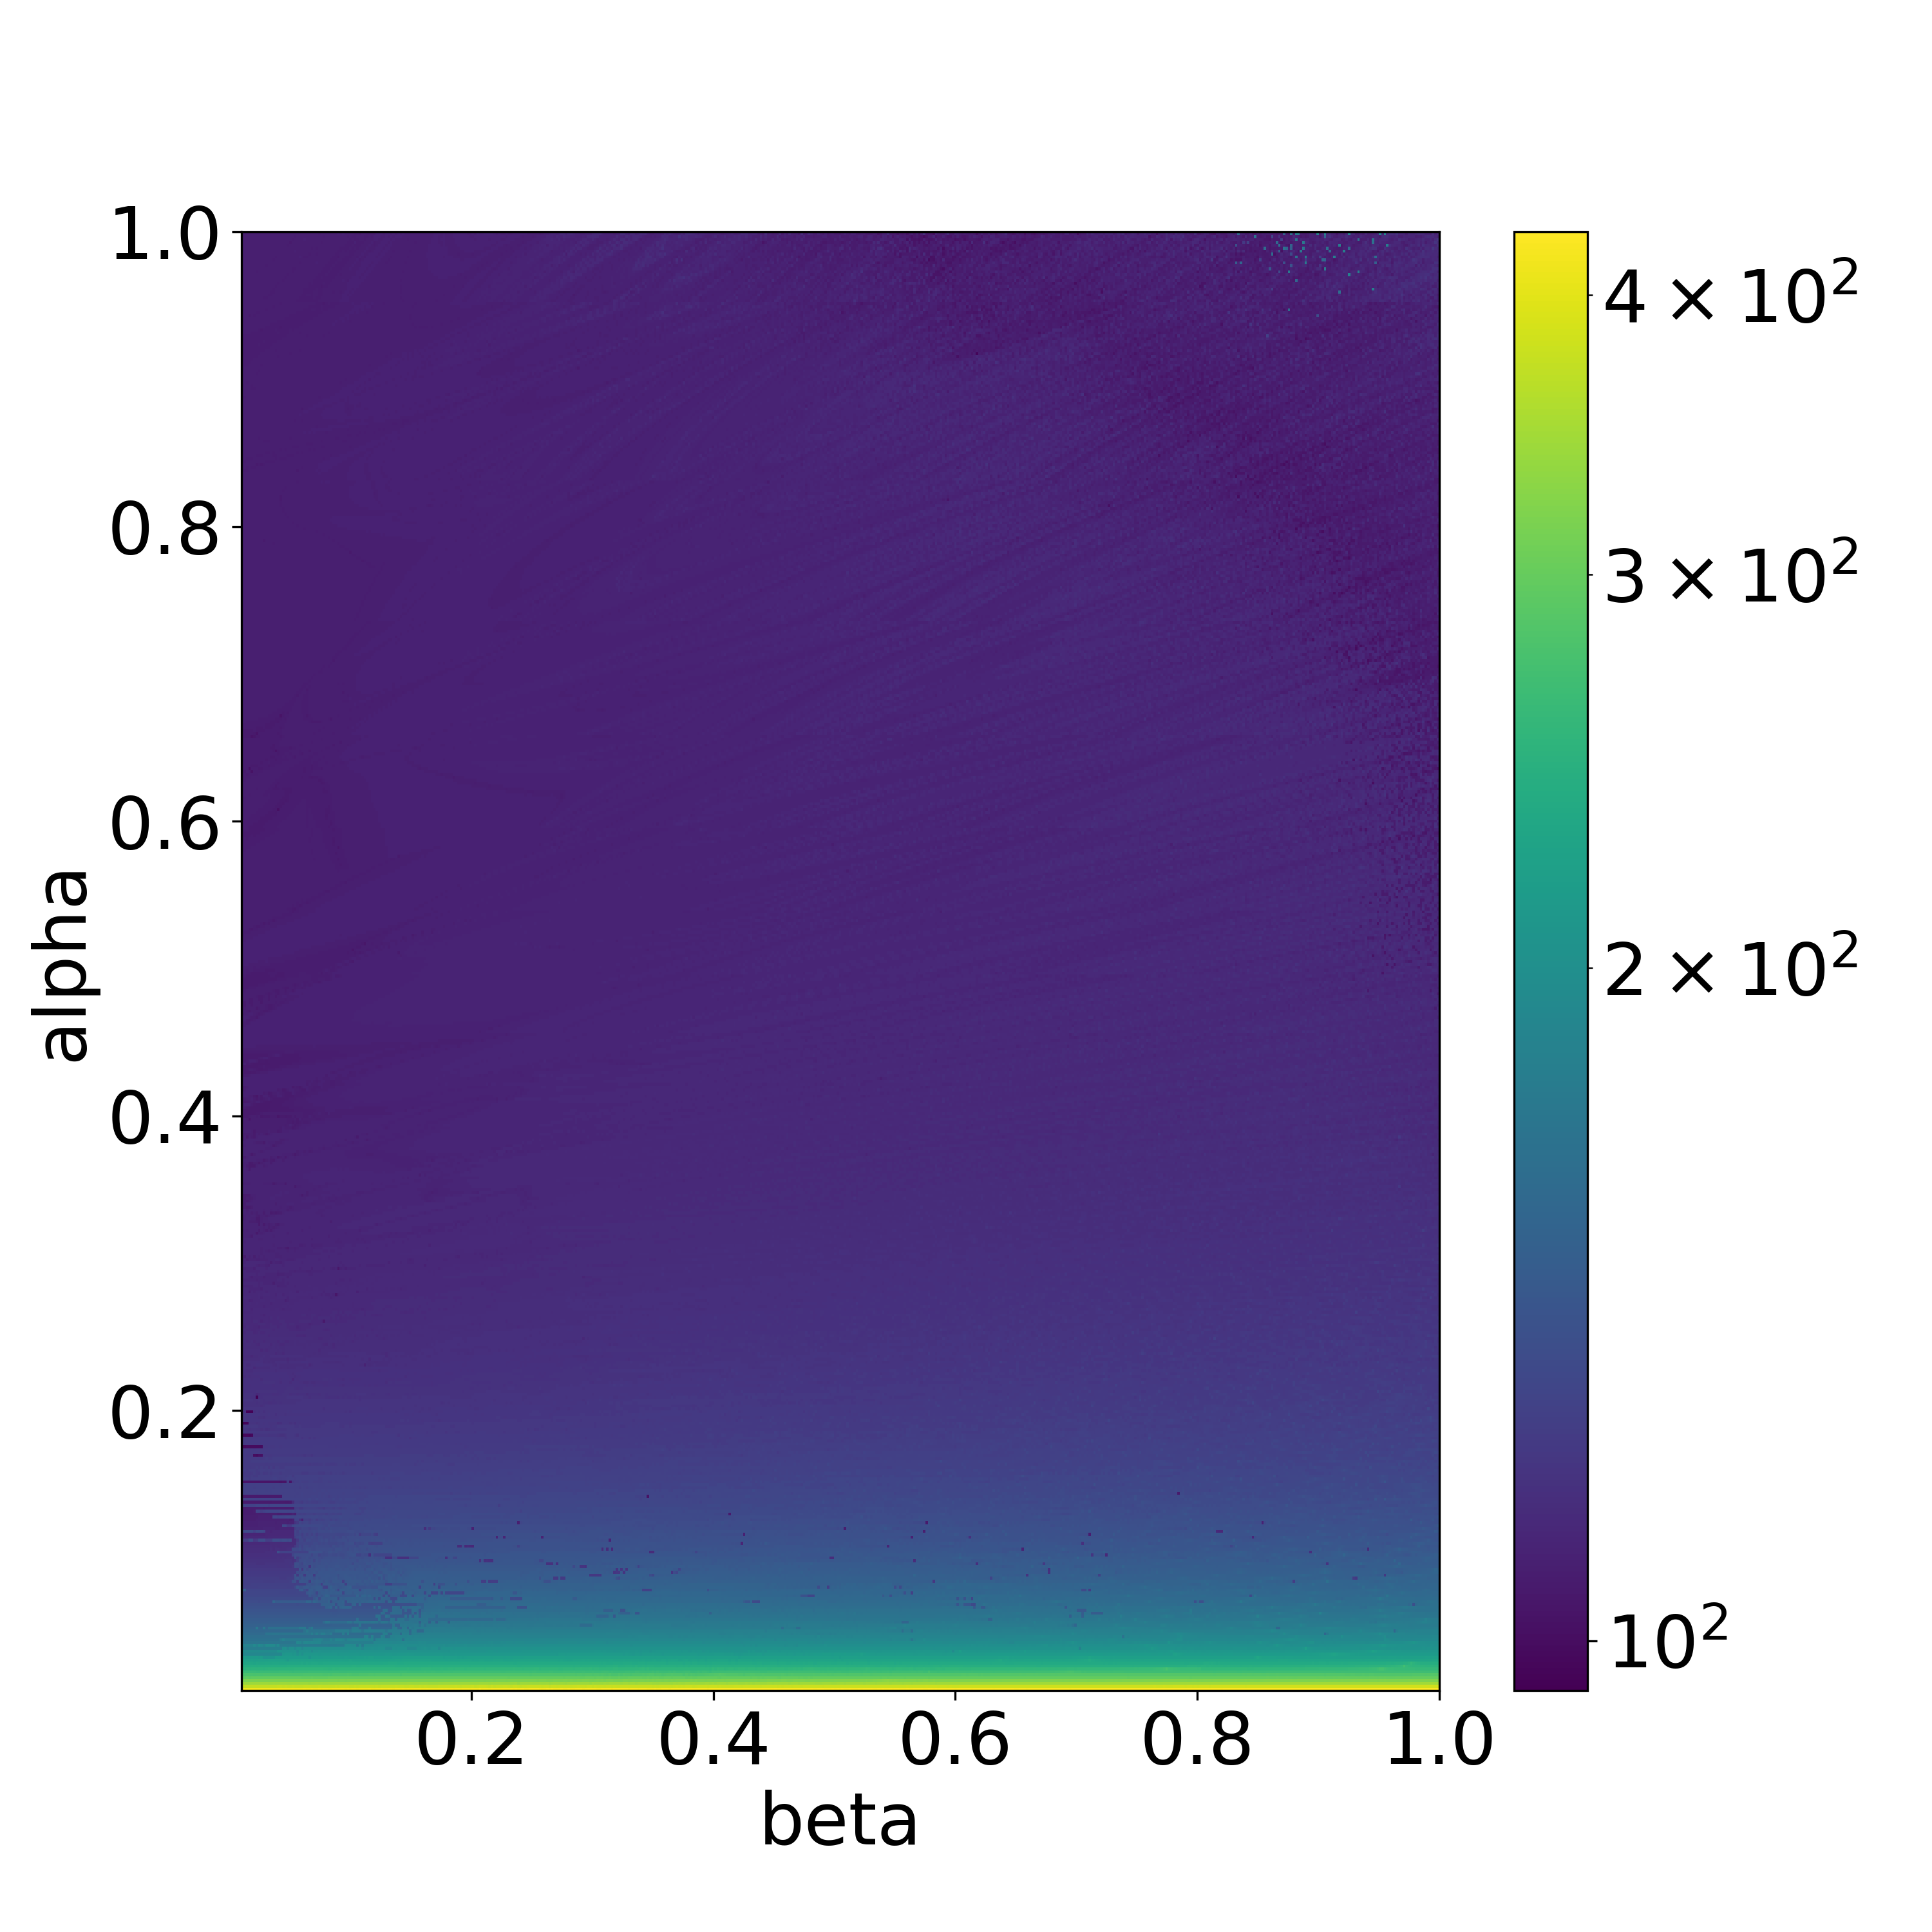
\includegraphics[width=0.28\textwidth]{images/analysis_RKF45_TS.png} & 
    	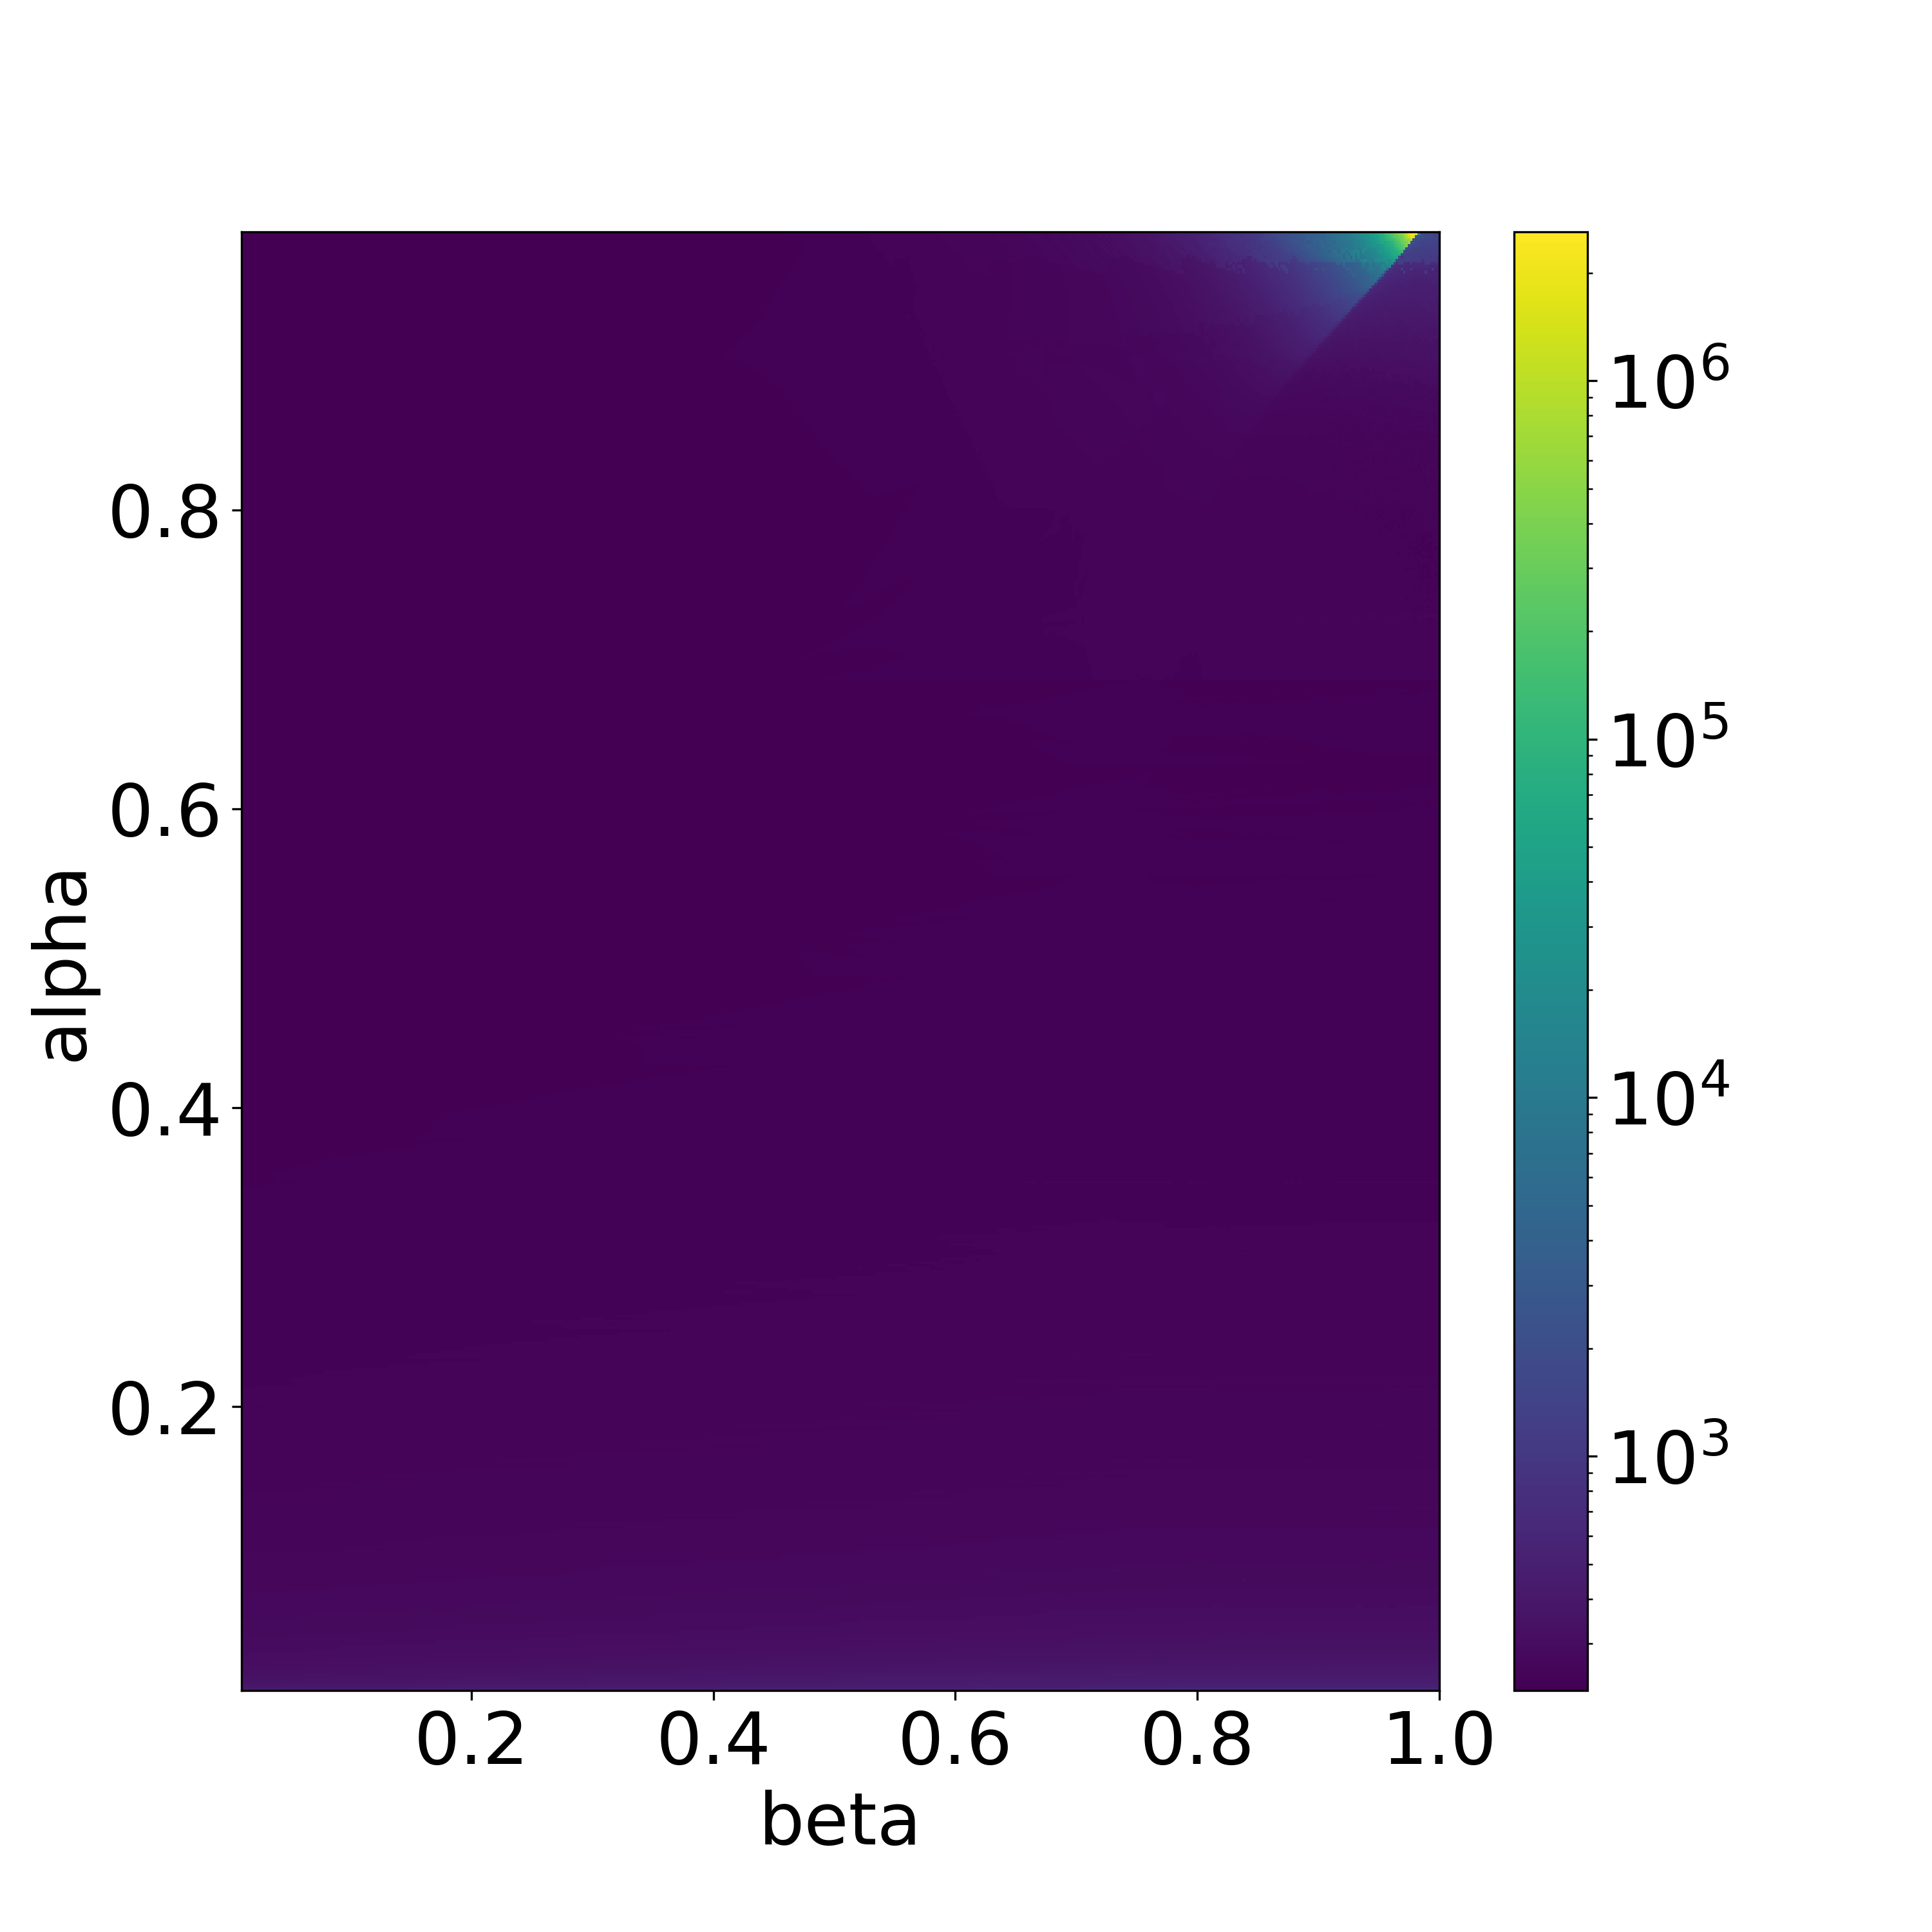
\includegraphics[width=0.28\textwidth]{images/analysis_BDF12_TS.png} & 
    	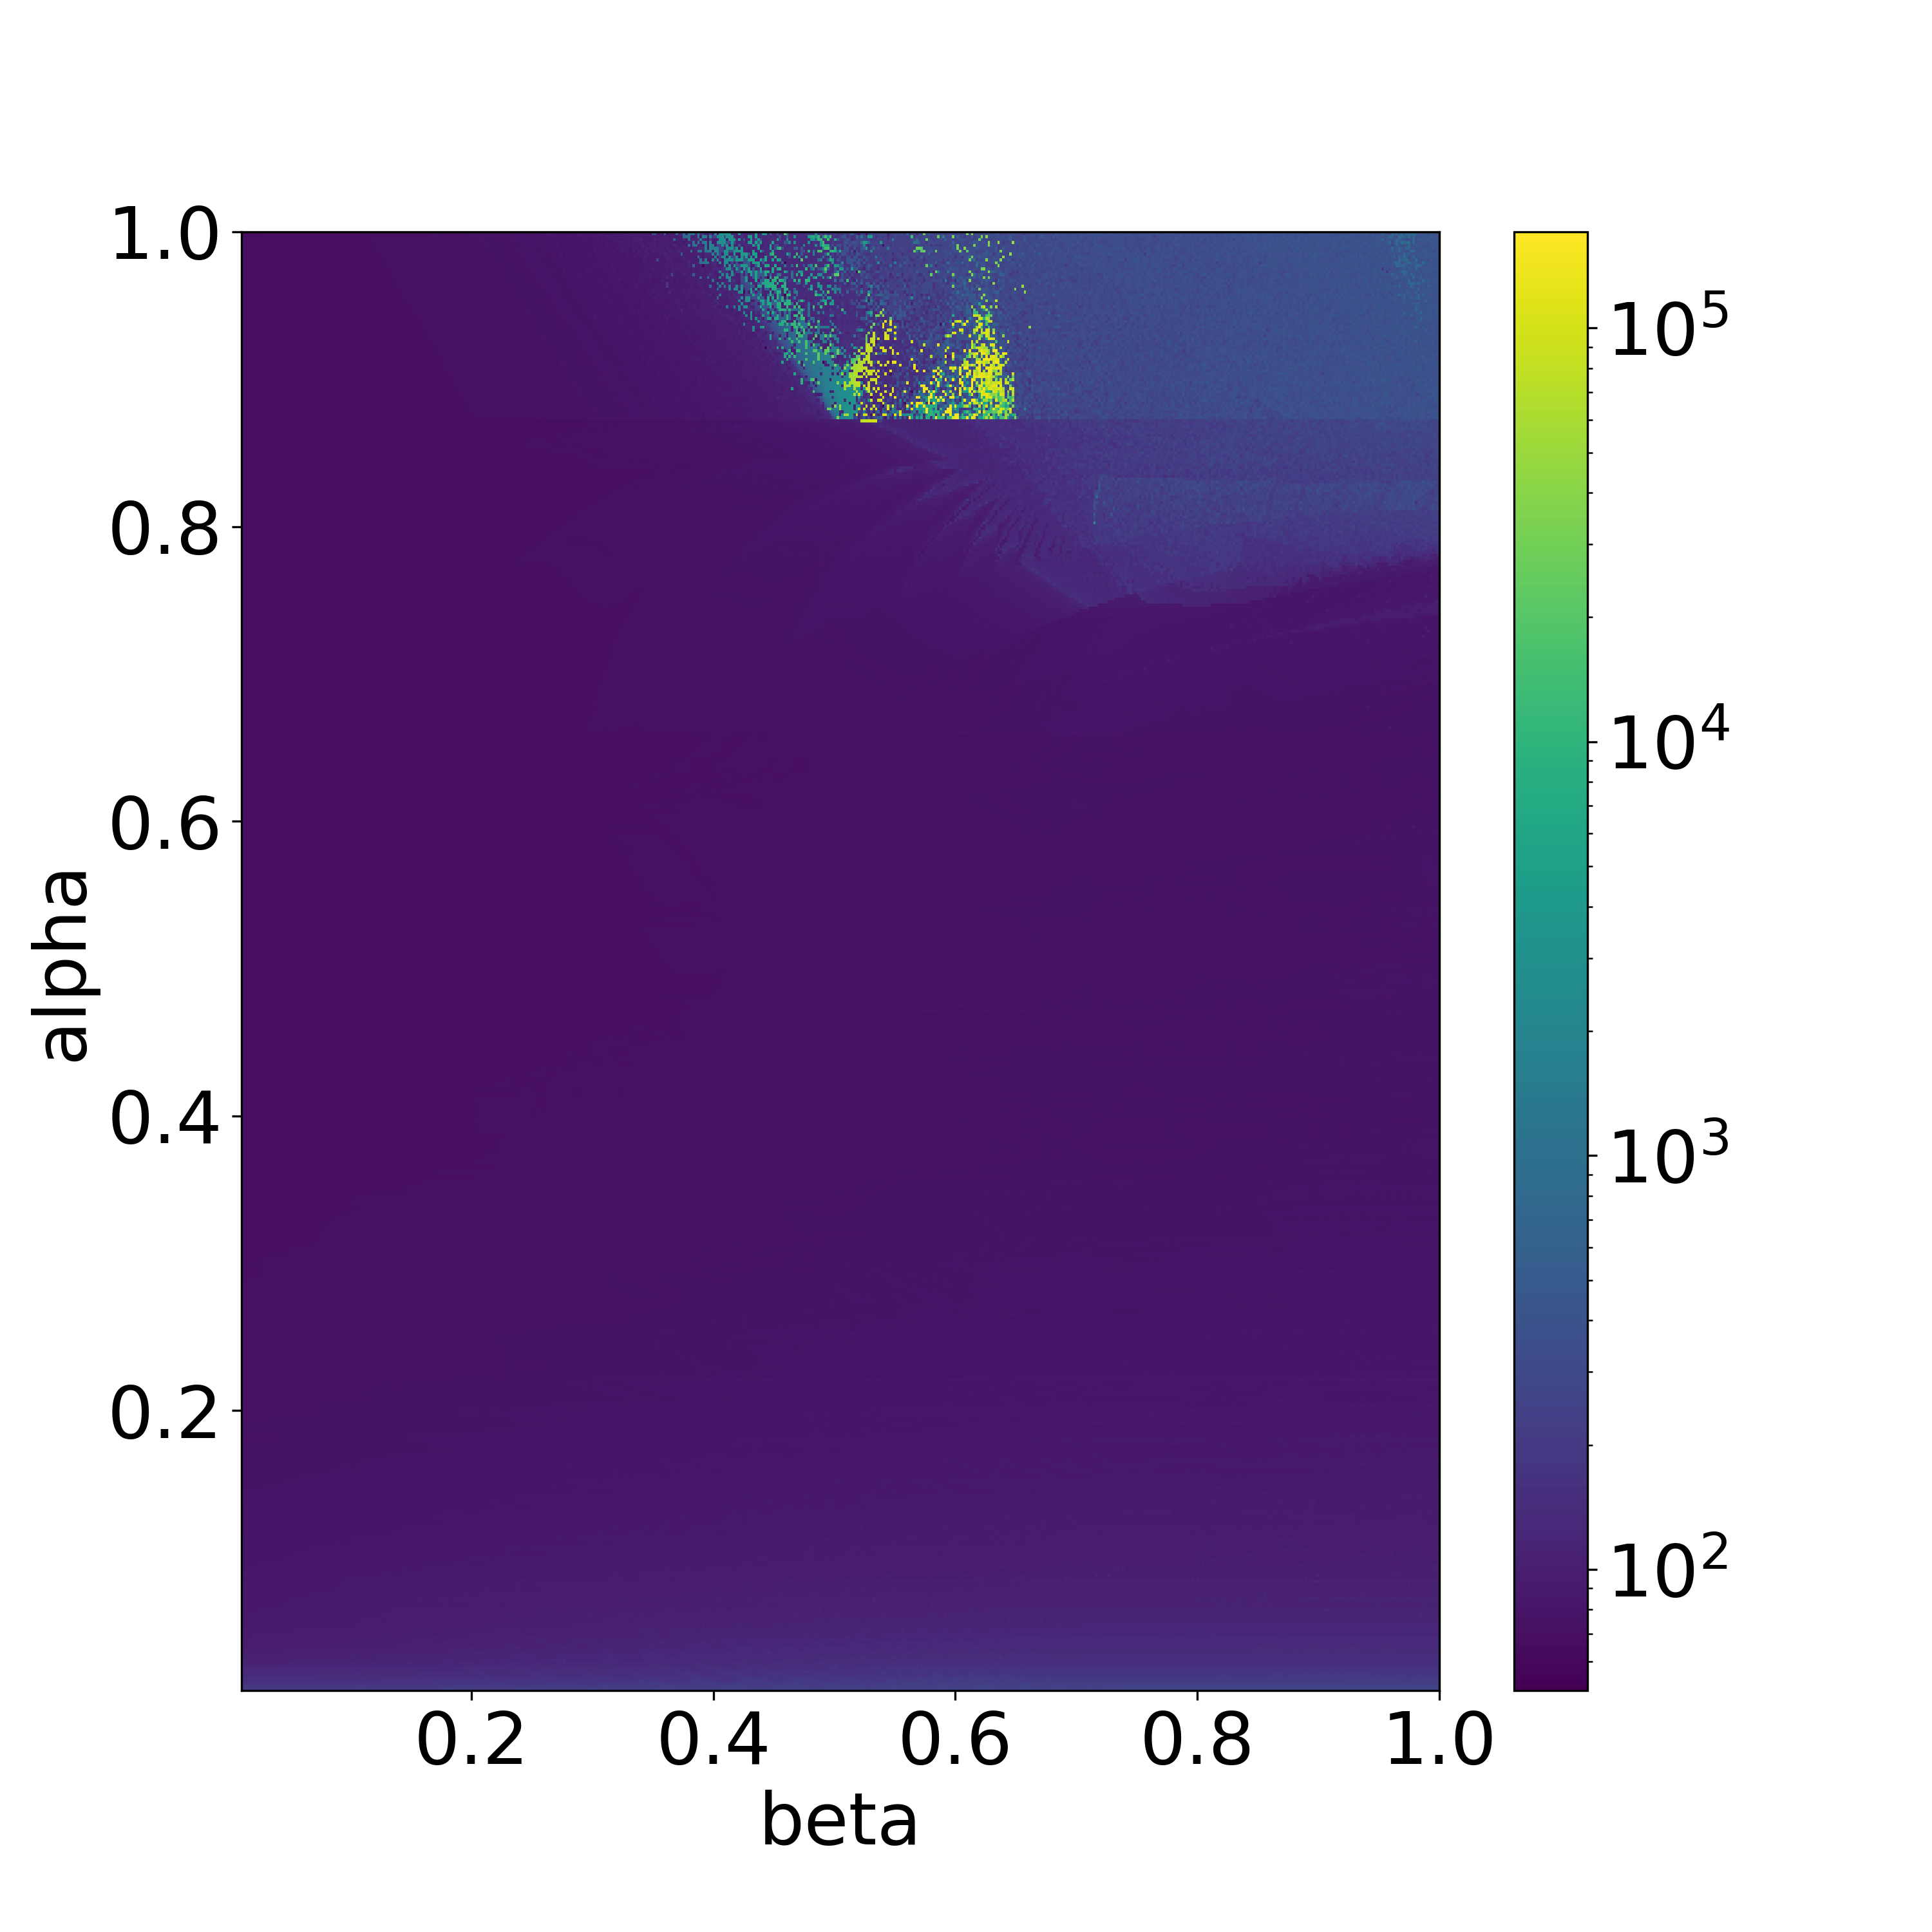
\includegraphics[width=0.31\textwidth]{images/analysis_BDF23_TS.png} \\
		\textbf{b} &
    	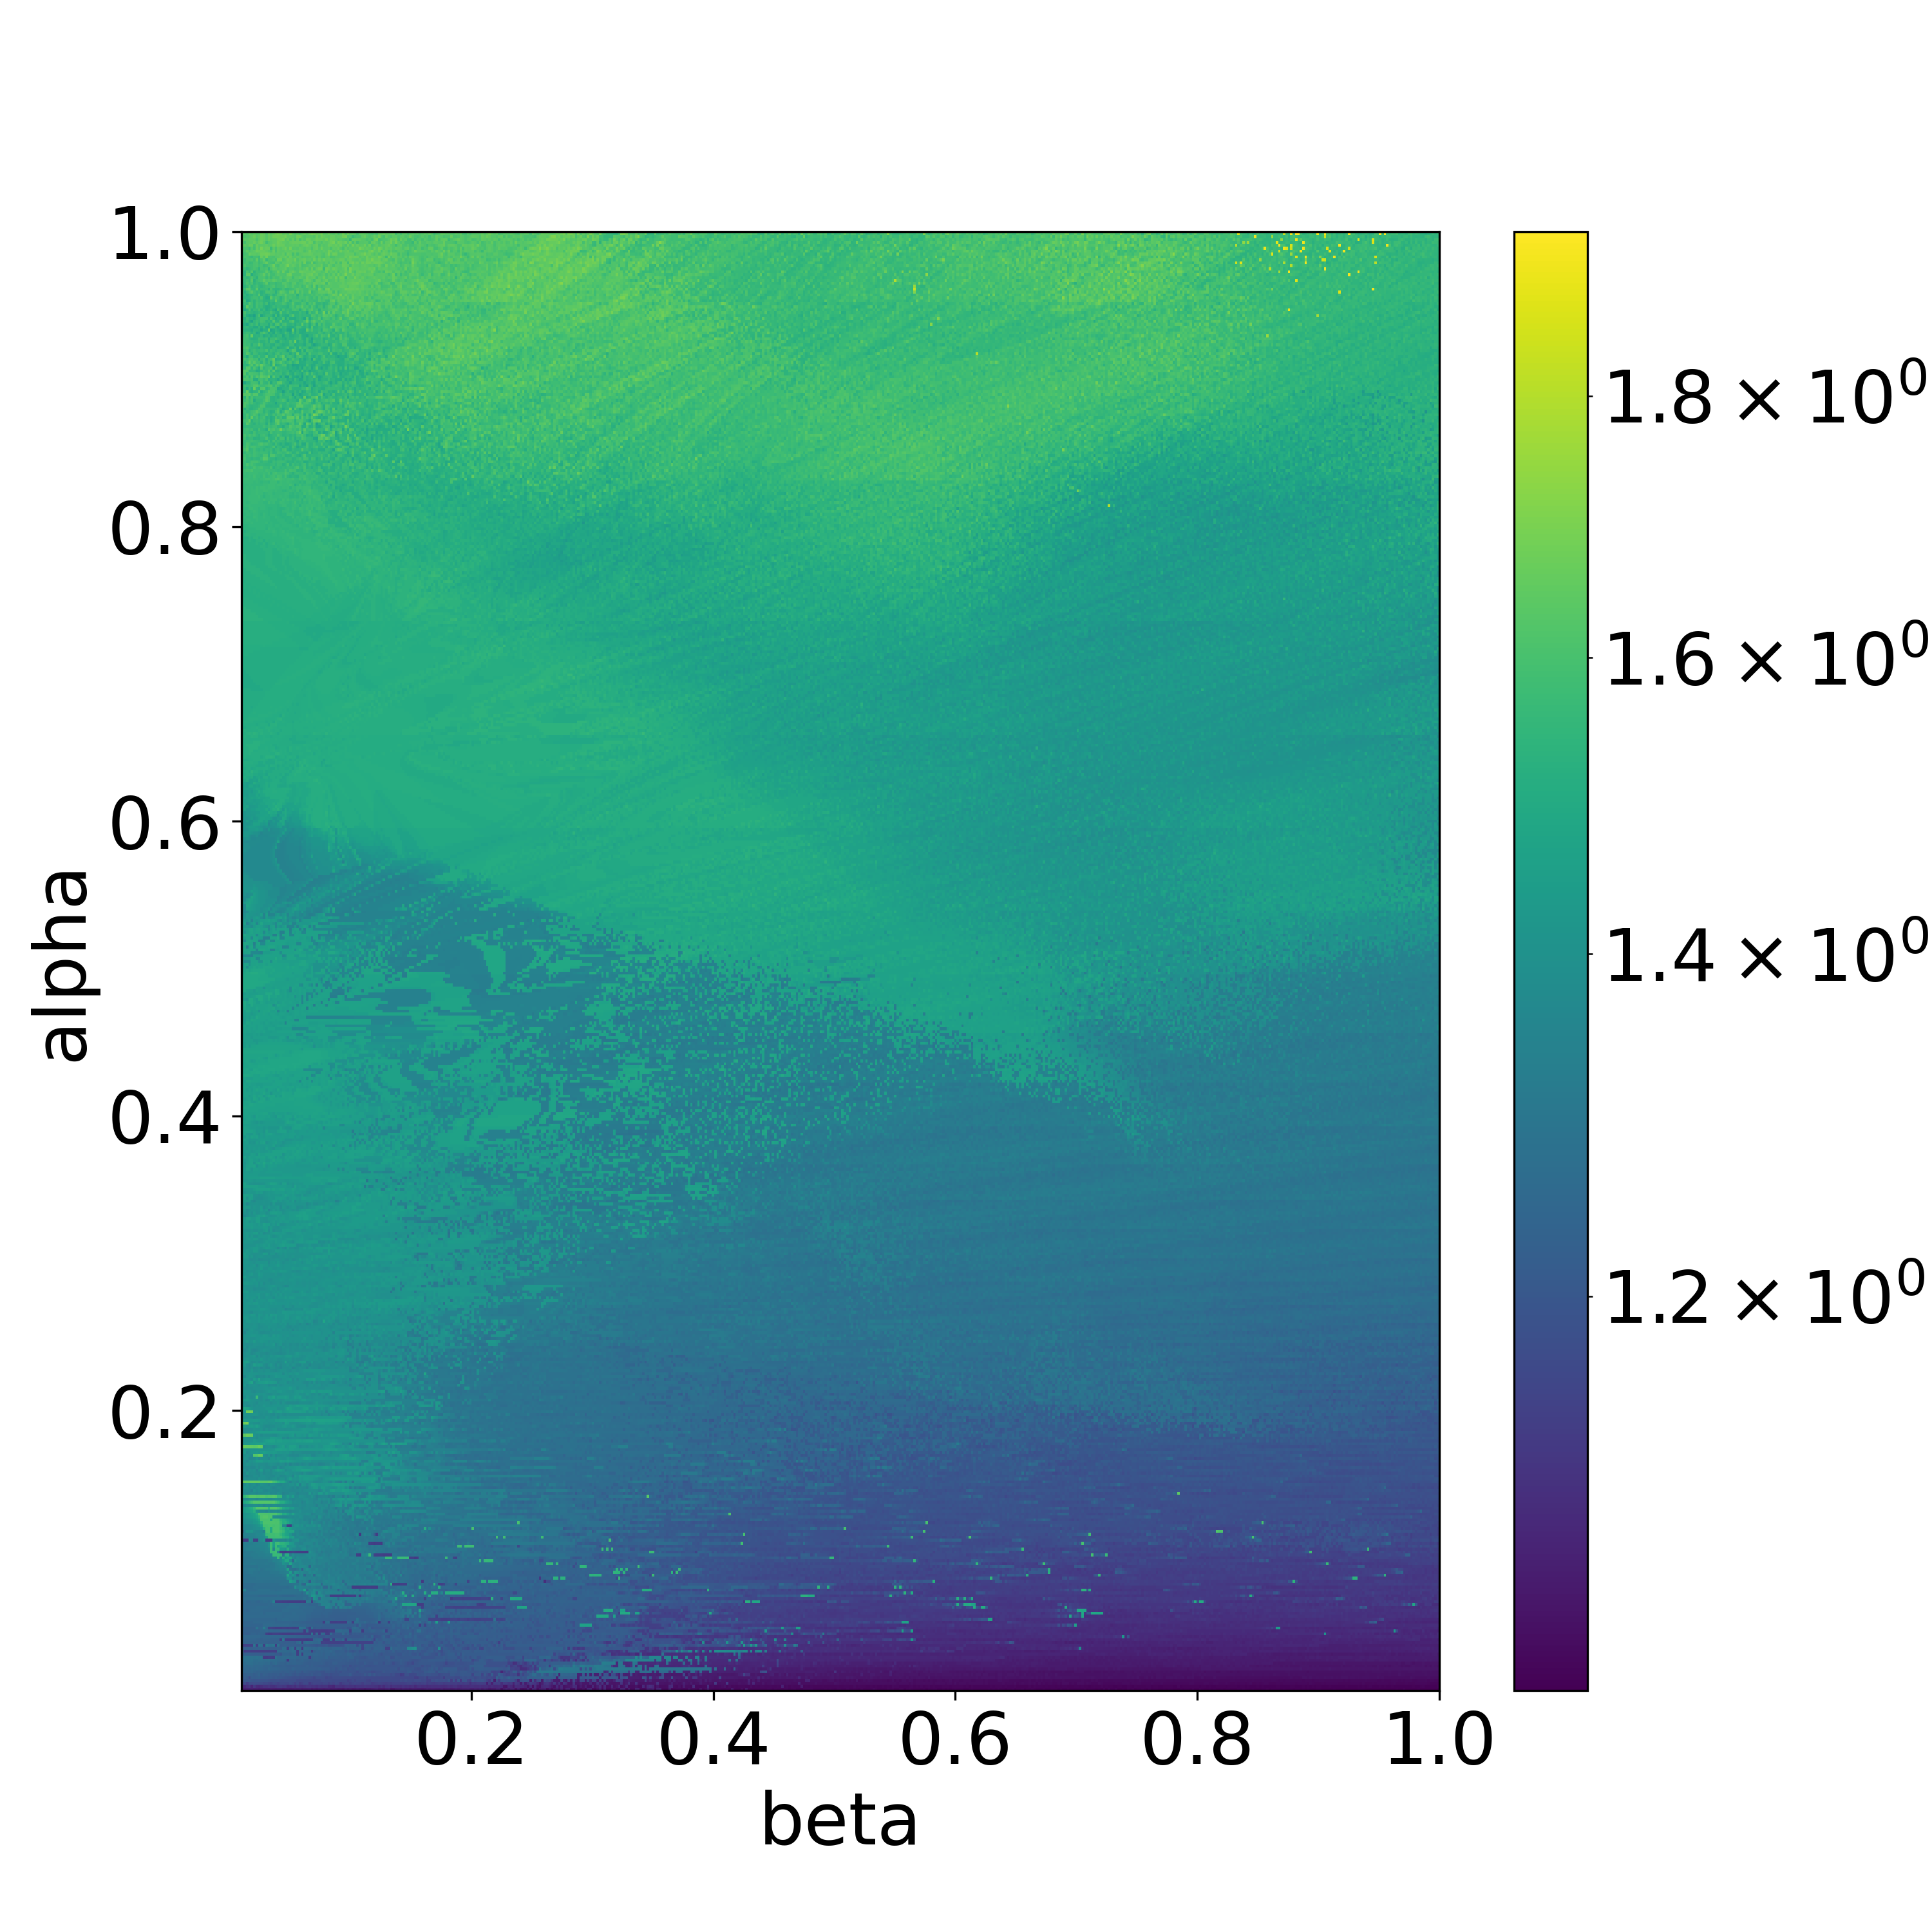
\includegraphics[width=0.28\textwidth]{images/analysis_RKF45_NI.png} &
		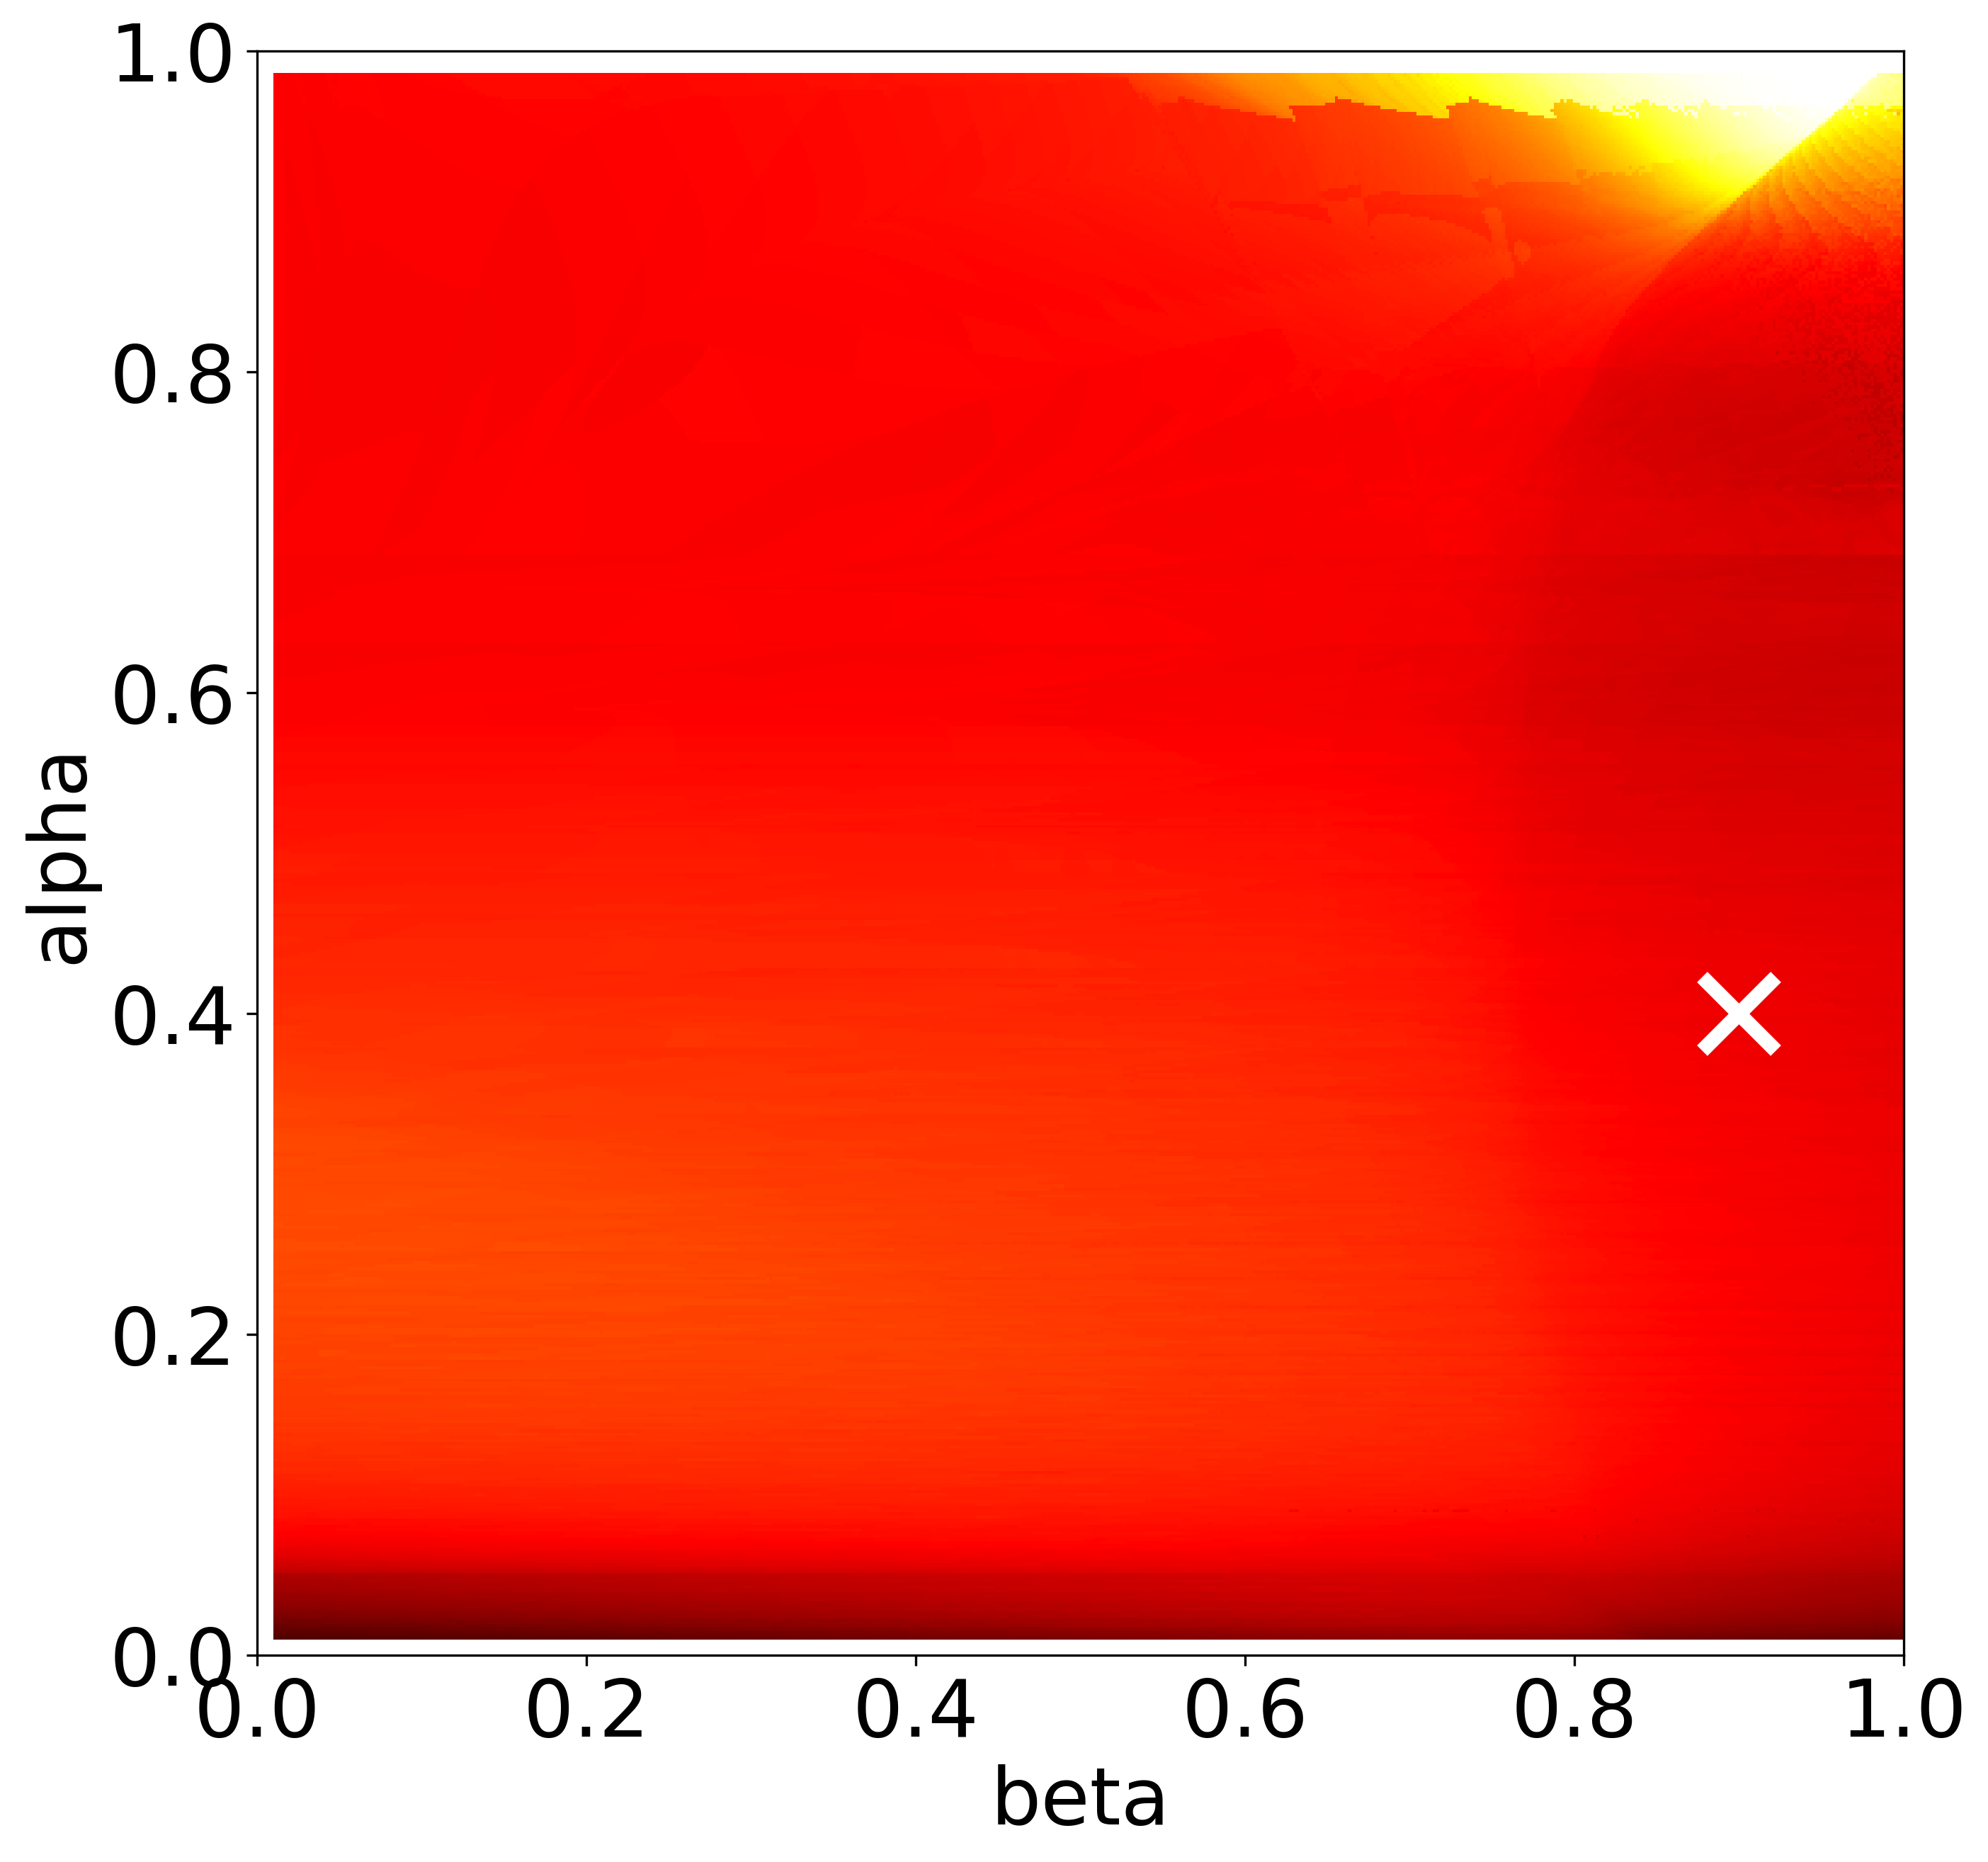
\includegraphics[width=0.28\textwidth]{images/analysis_BDF12_NI.png} &
		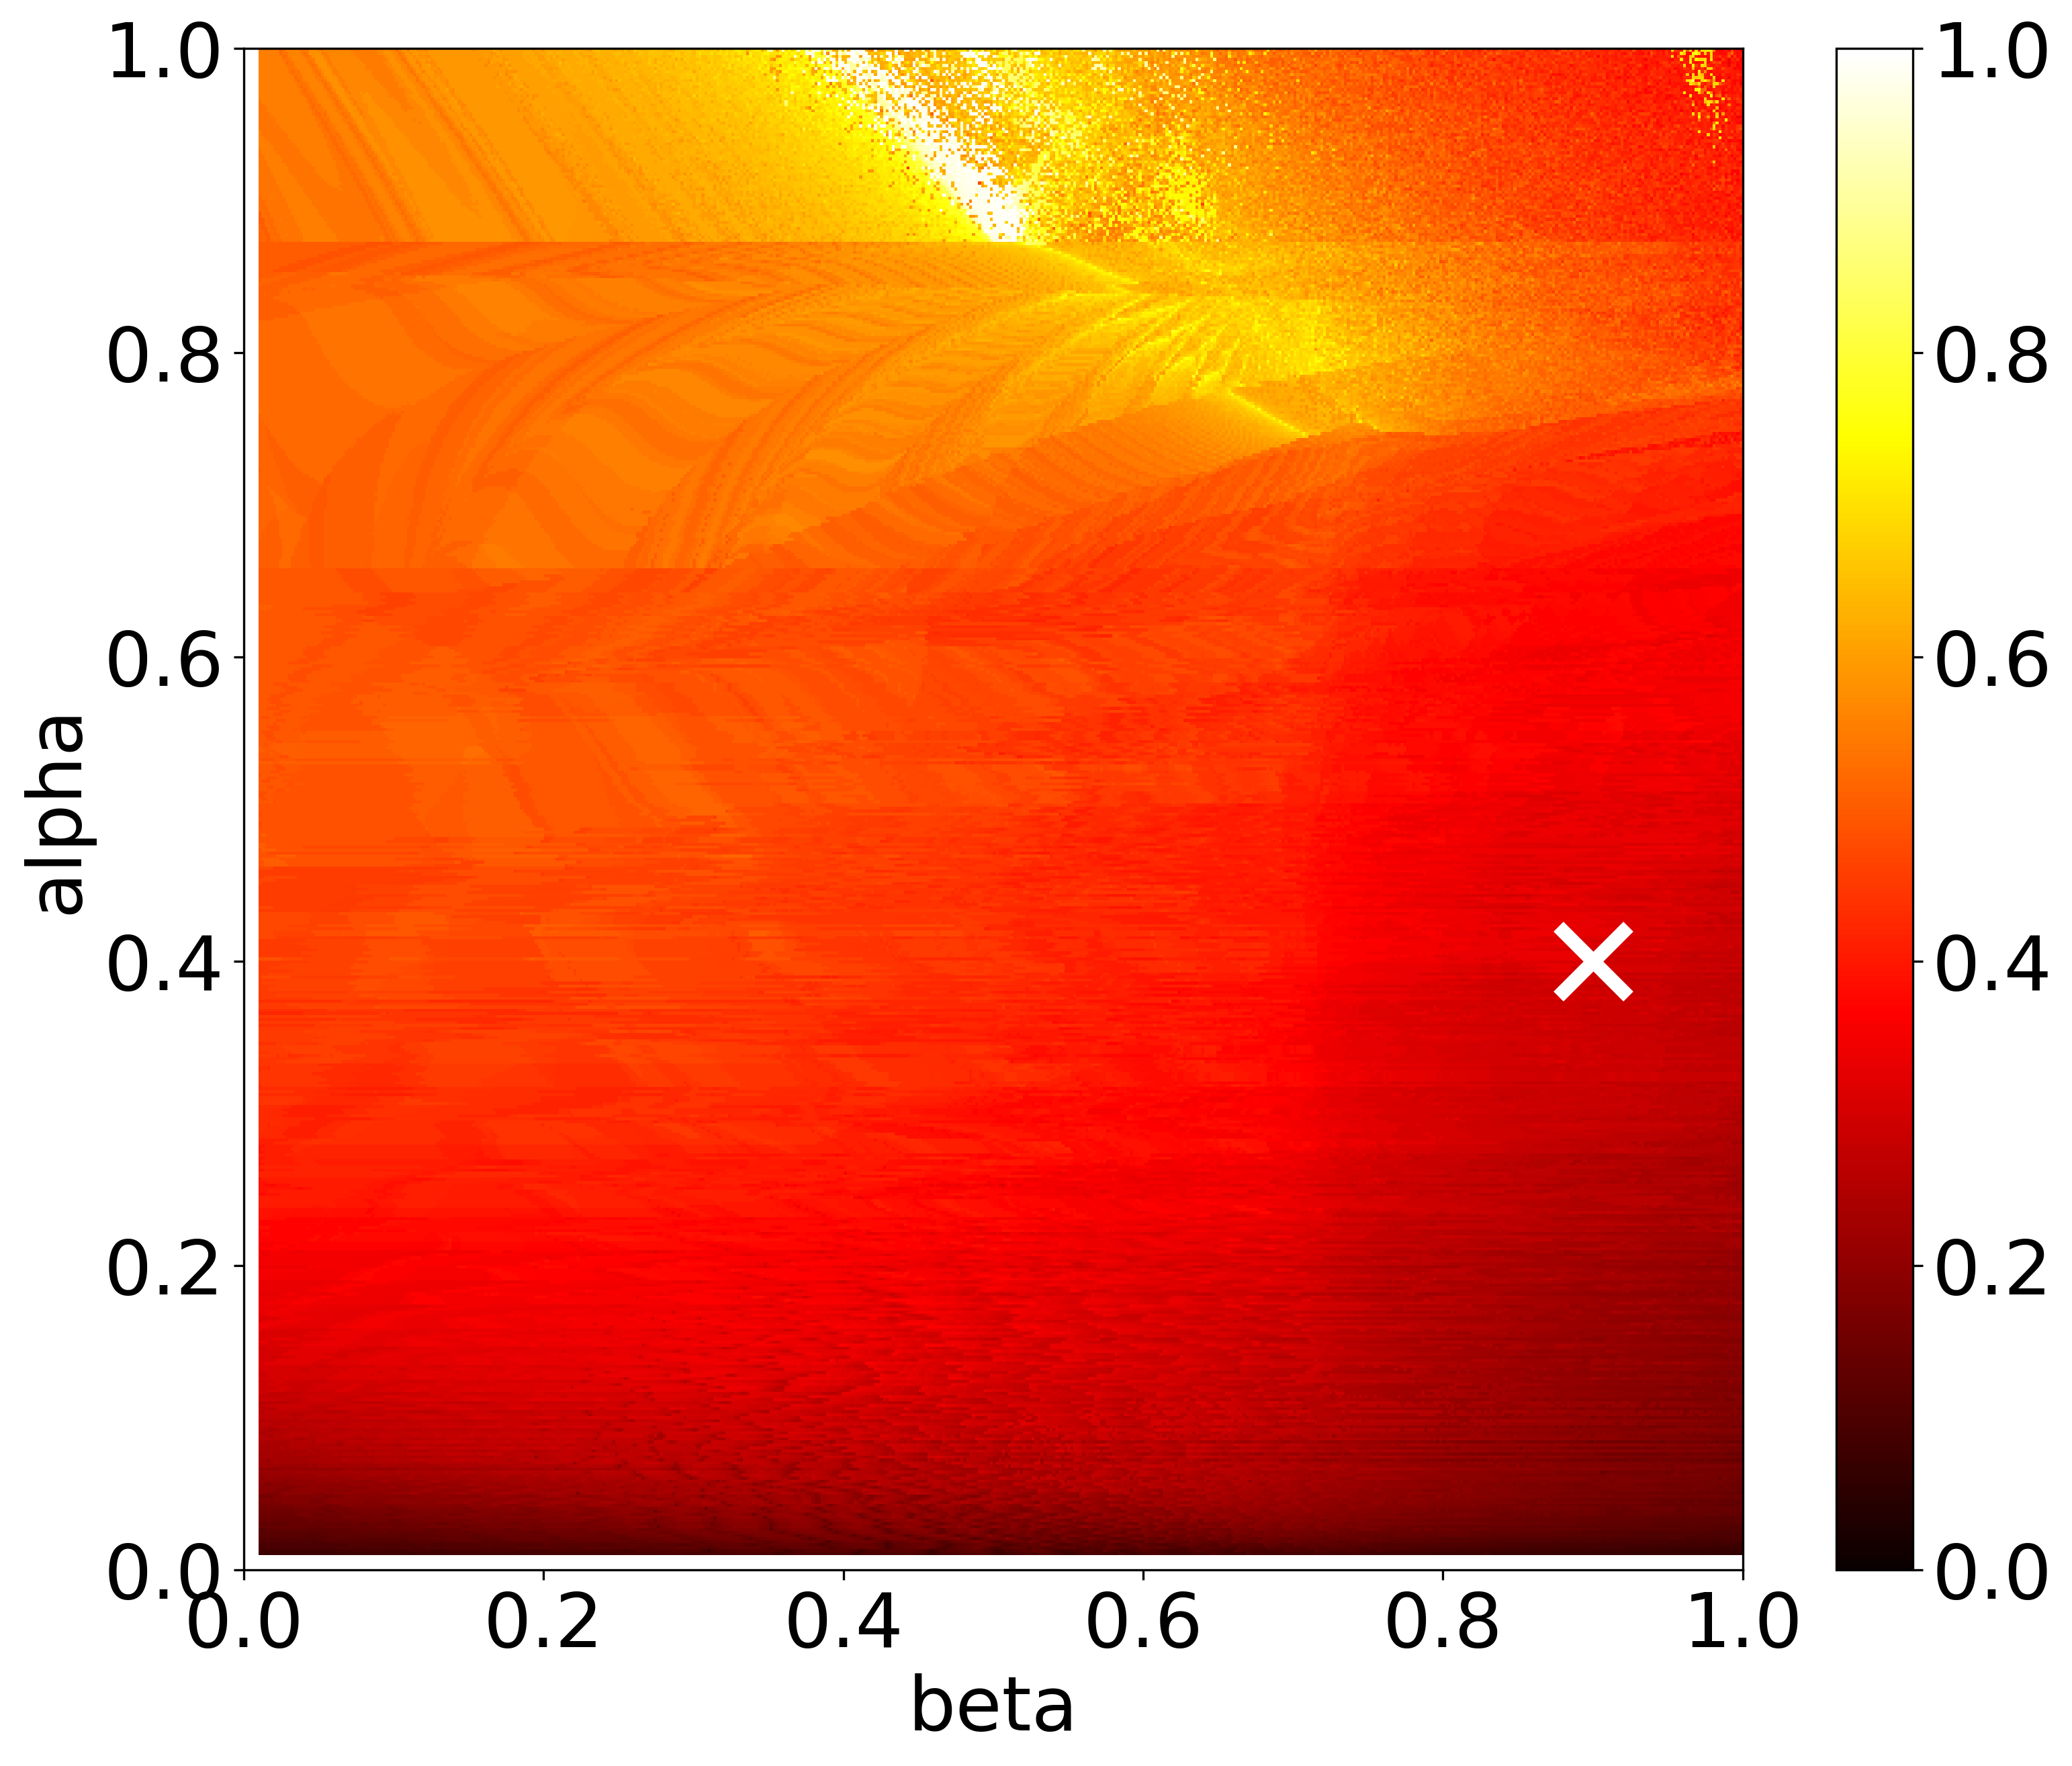
\includegraphics[width=0.31\textwidth]{images/analysis_BDF23_NI.png} \\
		\textbf{c} &
    	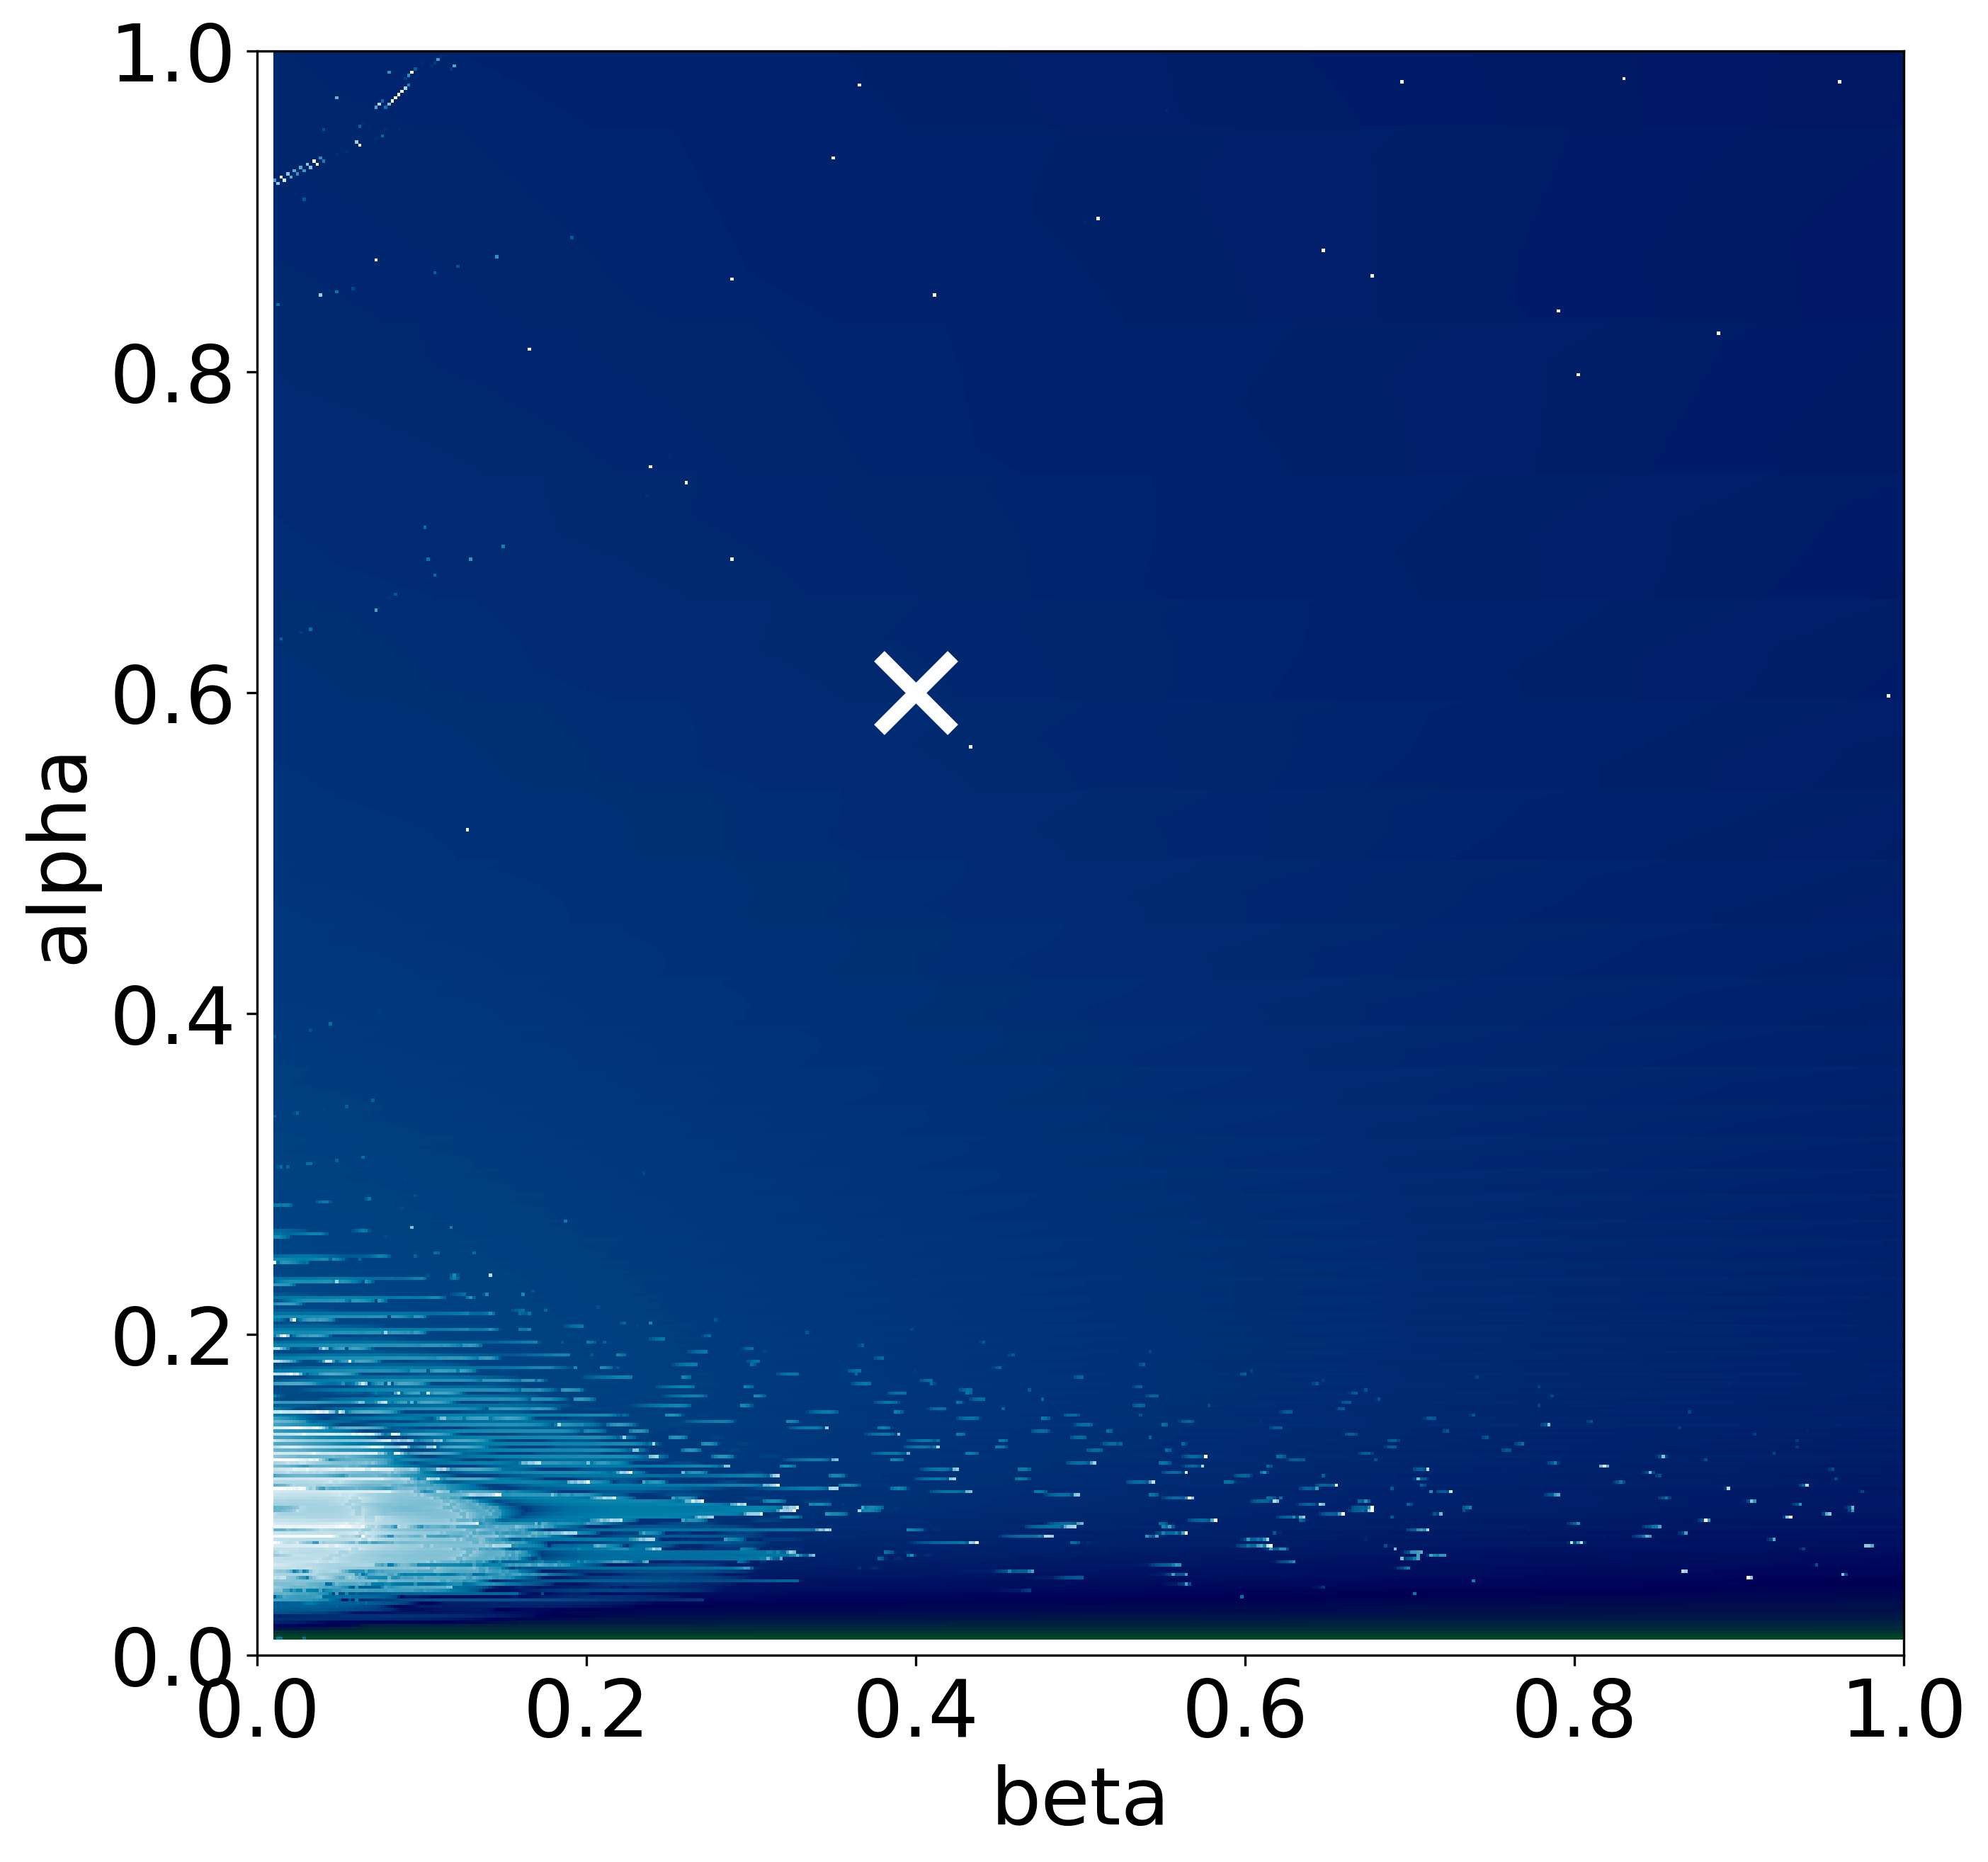
\includegraphics[width=0.28\textwidth]{images/analysis_RKF45_psi.png} &
		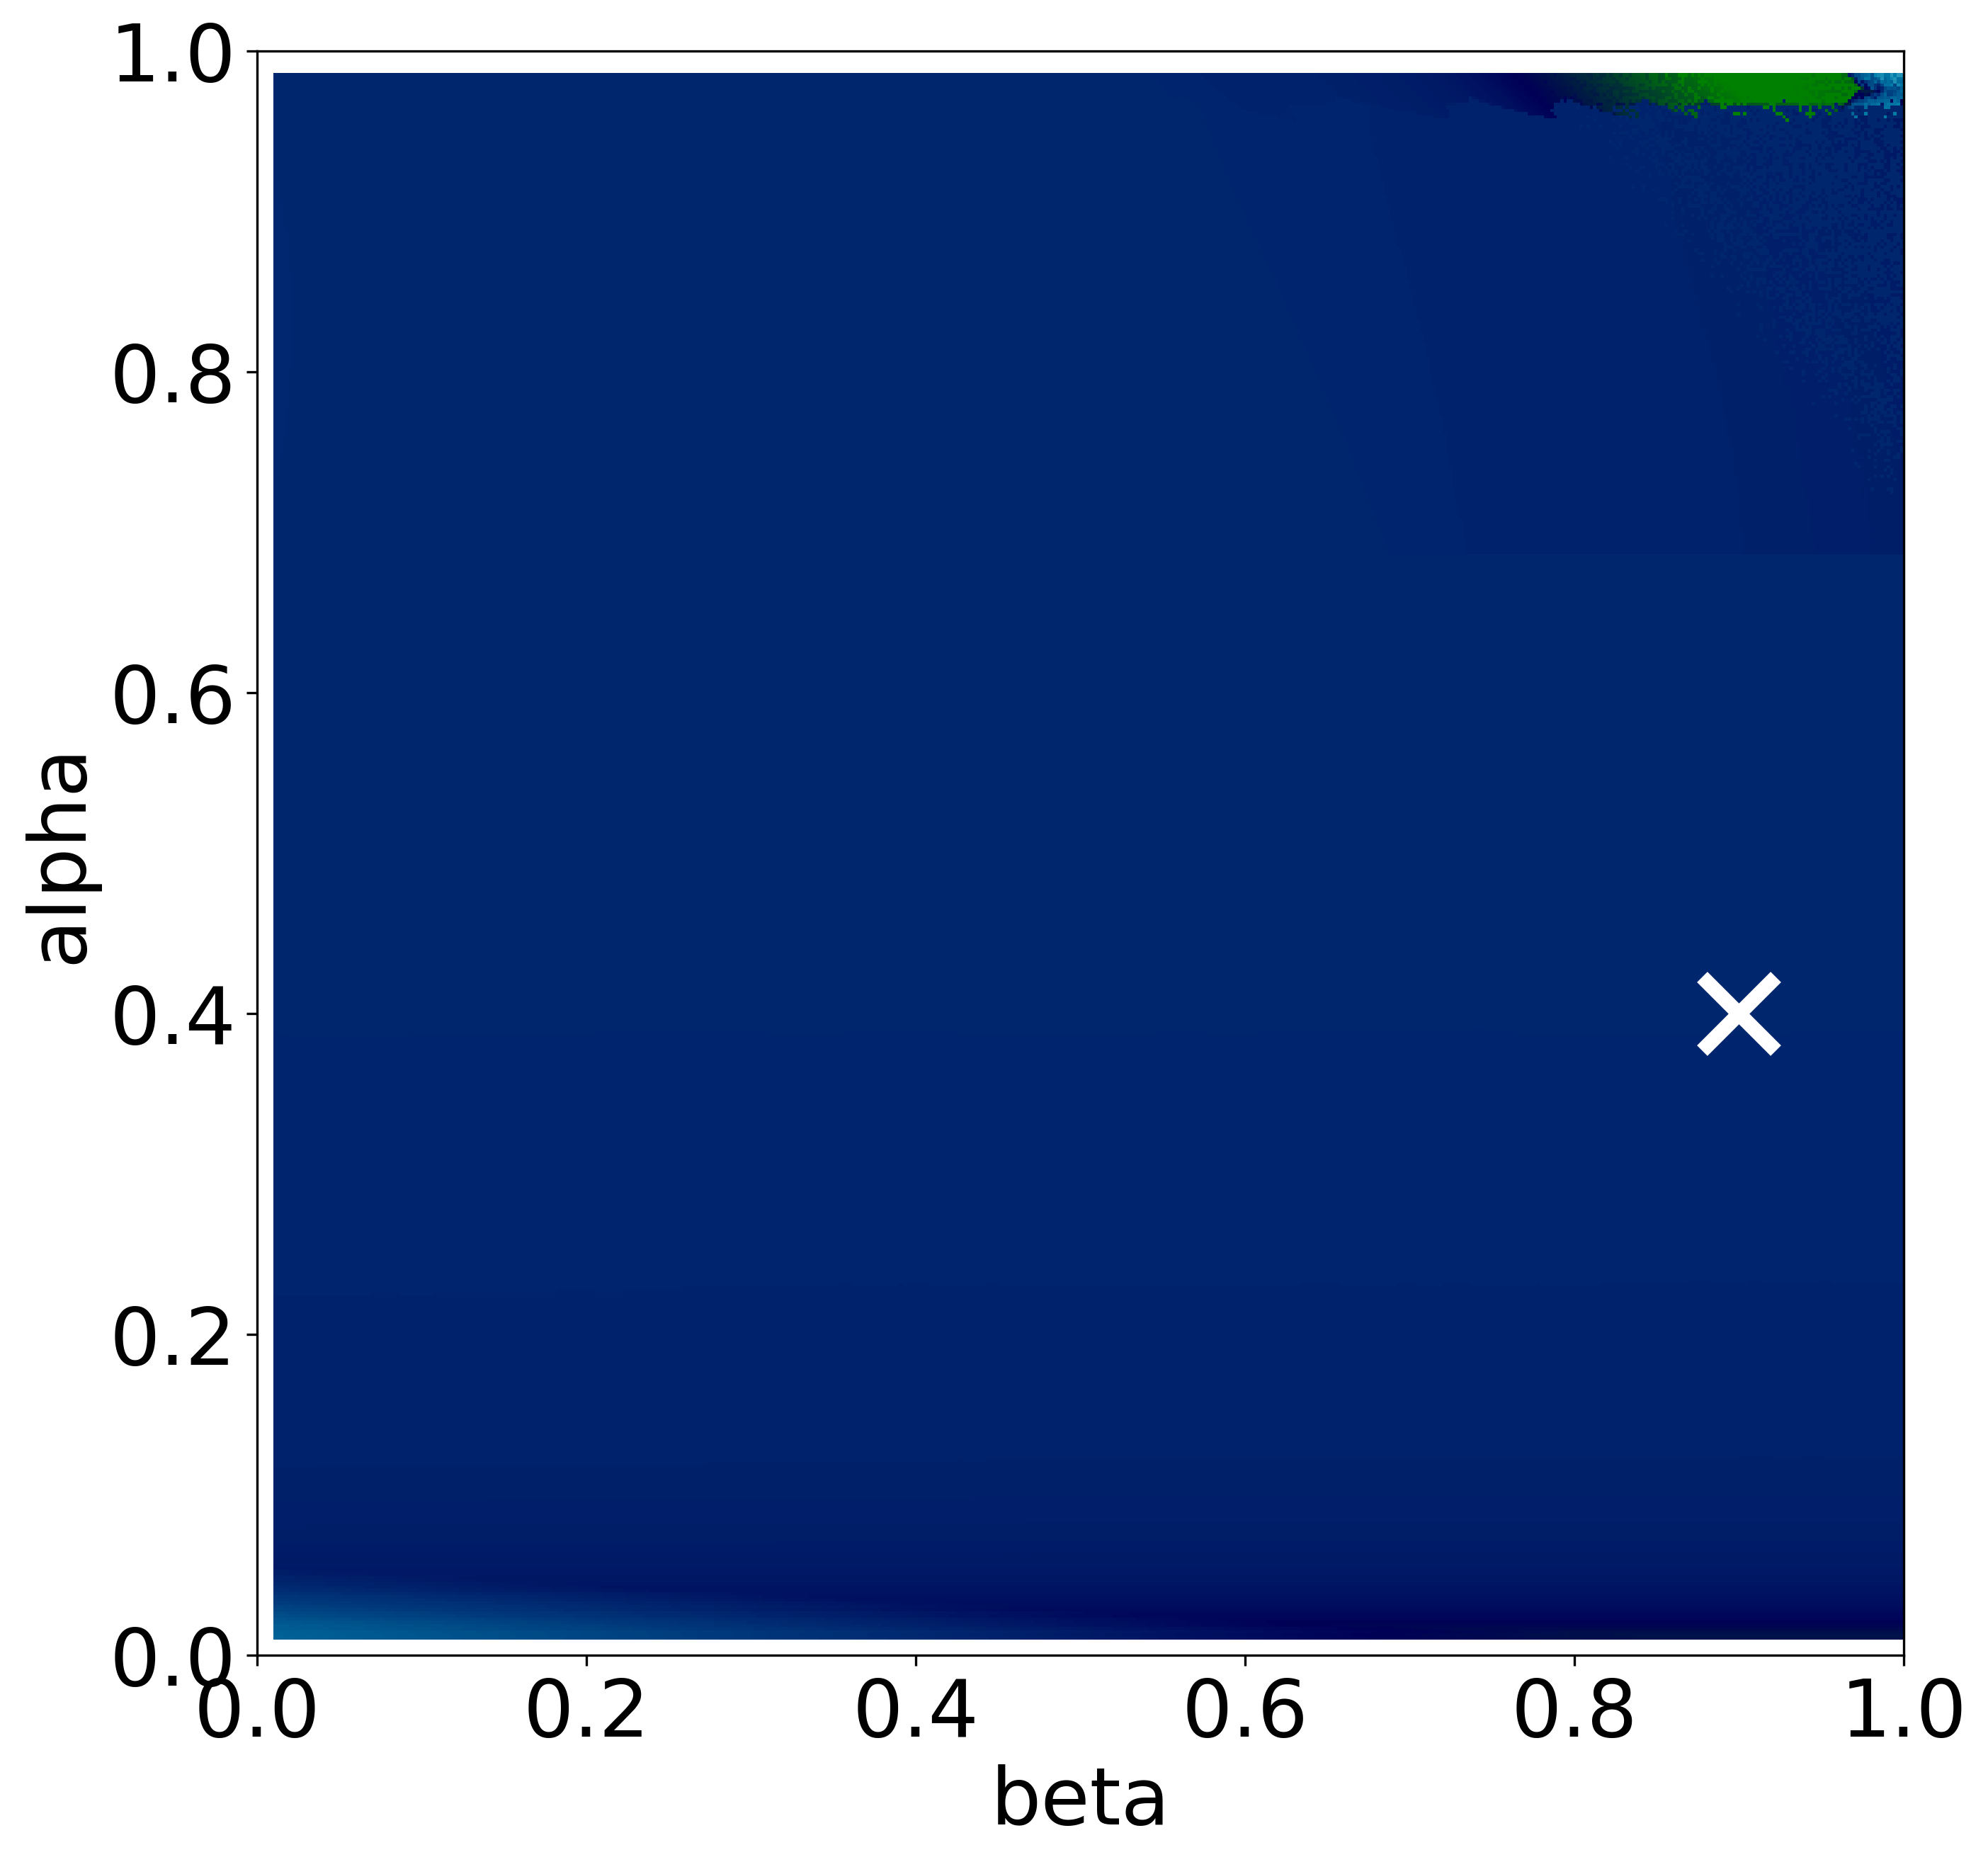
\includegraphics[width=0.28\textwidth]{images/analysis_BDF12_psi.png} &
		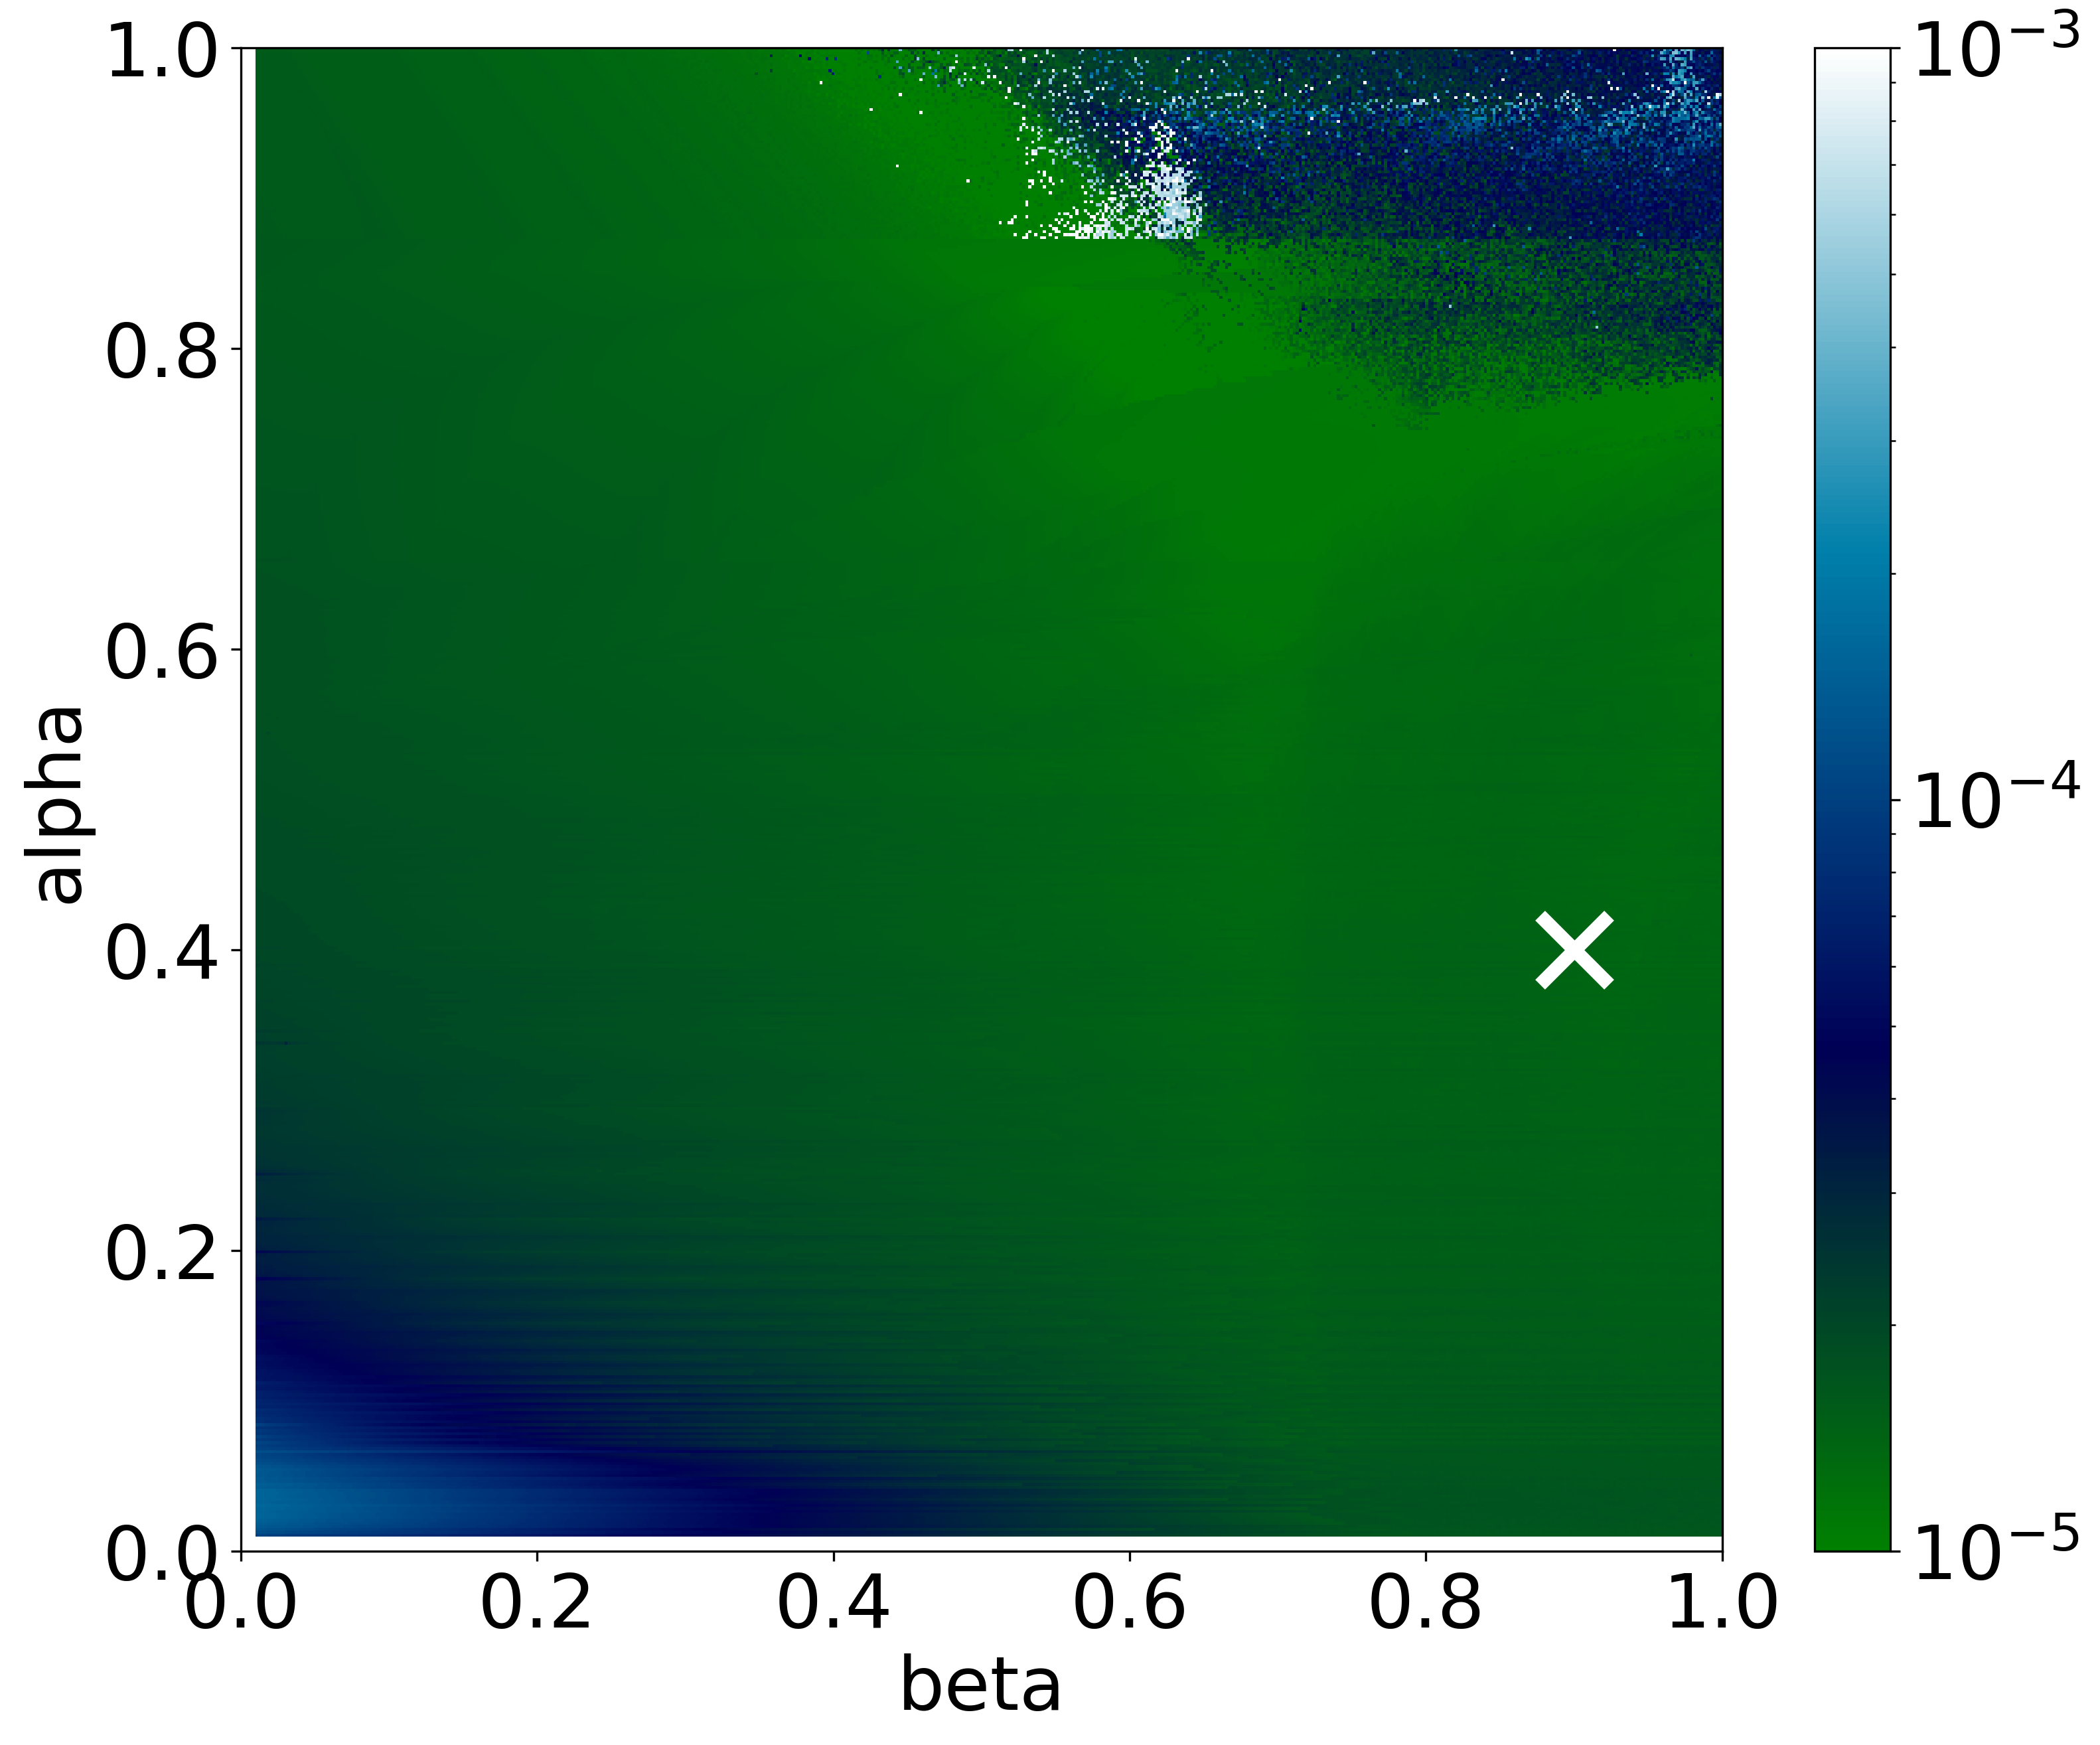
\includegraphics[width=0.32\textwidth]{images/analysis_BDF23_psi.png} \\
	\end{tabularx}
    \caption{Impact of the parameters $\alpha$ and $\beta$ of the PI controller on the number of required iterations to solve the model problem from \autoref{eq:first_DAE_ODE} for a simulation time of $t=5.0s$. The white crosses indicate the empirically found optimum. \\ \textbf{a}: Number of required timesteps \\ \textbf{b}:  Average number of step rejections \\ \textbf{c}: Absolute error of the variable $\bar{\psi}$ }
    \label{fig:ParametersPIController}
\end{figure}
There are now two design parameters $k_I$ and $k_P$ that have to be determined. Their ideal values depend on the considered problem and the picked numerical solver and one option is to find them empirically. The parameters can be expressed in function of the order of the numerical solver $k-1$ by $k_I = \alpha / k$ and $k_P = \beta / k$. For the three considered solvers (\textbf{RKF4}, \textbf{BDF1} and \textbf{BDF2}), the total amount of timesteps is measured for varying values of $\alpha$ and $\beta$. It may also occur that the estimated error exceeds the tolerance, in this case the step is rejected and repeated with a lower timestep size. In the ideal case, the number of step rejections is zero. The results are shown in \autoref{fig:ParametersPIController}. The tolerance for the local truncation error estimate has been set to $t=1\cdot 10^{-6}$ to ensure convergence of all numerical schemes and thus obtain comparable results. \\

Ideal parameters $\alpha$ and $\beta$ minimize the number of required timesteps, and keep the number of step rejections as low as possible. Further, the error in $\bar{\psi}$ should not be too large. From the observations in the graphs above, we choose as parameters:
\begin{itemize}
    \item for \textbf{RKF4}: $\alpha=0.4$ and $\beta=0.6$
    \item for \textbf{BDF1}: $\alpha=0.9$ and $\beta=0.4$
    \item for \textbf{BDF2}: $\alpha=0.9$ and $\beta=0.4$
\end{itemize}

\subsection{Comparison between the timestep contollers}
The elementary local error controller corresponds to the PI-controller with parameters $\alpha = 1$ and $\beta=0$. It seems that in the graphs above, the color at the ideal parameters and in the upper-left corner are mostly similar. Indeed, the errors are almost the same, and the total number of step execution, calculated as the product of the total timestep number and the number of iterations per step, could only be decreased by 7\% with the PI controller. In the continuation of the thesis, only the elementary local error controller will be used, which is the default implementation in PETSc. 

\section{Comparison between numerical schemes}
So far, one explicit (\textbf{RKF4}) and two implicit (\textbf{BDF1}, \textbf{BDF2}) numerical solvers have been implemented for the initial DAE in \autoref{eq:first_DAE_algeb} and their respective ideal parameter choice for their use with a PI controller has been discussed. Now, the quality of the solutions is compared. \\

\subsection{Numerical solutions}
Again, the allowed tolerance of the PI controller is set to $t=10^{-6}$. The method of the manufactured solutions is chosen to have an analytical solution against which numerical computations can be compared. The parameters $t_e$ and $t_w$ are chosen in a way that the velocity is initially close to zero and increases to one within one second at the middle of the simulation time. \autoref{fig:timeEvolutionValues} depicts the solution variables $\bar{\psi}$ and $V$ over time for all three solvers. The expected form of the $atan$ function centered around $2.5$ for the velocity is obtained with all methods and the results for $\bar{\psi}$ match too, as $\bar{\psi}$ decreases linearly before it stabilizes around zero as the velocity increases. \\
If adaptive timestepping methods are used, the actual size of the timestep $h_n$ is of particular interest. Since at each timestep, the right-hand side of the ODE and the algebraic equation have to be solved a fixed number of times, a method that allows larger timesteps is considered more efficient. As shown in \autoref{fig:timeEvolutionDT}, this metric varies greatly with the chosen numerical solver. The simulation time can be roughly split into three sections: The first phase corresponds to low velocity and decreasing $\bar{\psi}$ until the time $t=2.0s$. In it, the \textbf{RKF4} and \textbf{BDF2} methods allow for rather similarly large timestep sizes, whereas the \textbf{BDF1} method is restricted to timestep sizes which are about fives times smaller. The second phase is marked by the fast increase in velocity and the stabilization of $\bar{\psi}$. Such rapid changes in the solution should imply shorter timesteps to obtain accurate solutions, especially for \textbf{RKF4}, because explicit schemes face stability issues for stiff problems. Indeed, a decrease in the timestep size can be observed for all three methods, however, the explicit \textbf{RKF4} performs much better than expected with timesteps that are about twice as long as using \textbf{BDF2}. As previously, \textbf{BDF1} has the worst performance of all three methods which much smaller timesteps. In the last phase, when the velocity approaches 1 and $\bar{\psi}$ remains close to 0, the two implicit BDF methods reach very large timesteps with an increasing trend, whereas the timesteps generated by the controller \textbf{RKF4} stagnate at a rather low value. Overall, \textbf{BDF2} performs best with 69 timesteps, followed by \textbf{RKF4} with 120 and finally \textbf{BDF1} needs 230 timesteps to execute the whole simulation. 


\begin{figure}[H]
    \centering
    \begin{subfigure}{0.43\textwidth}
    	\centering
    	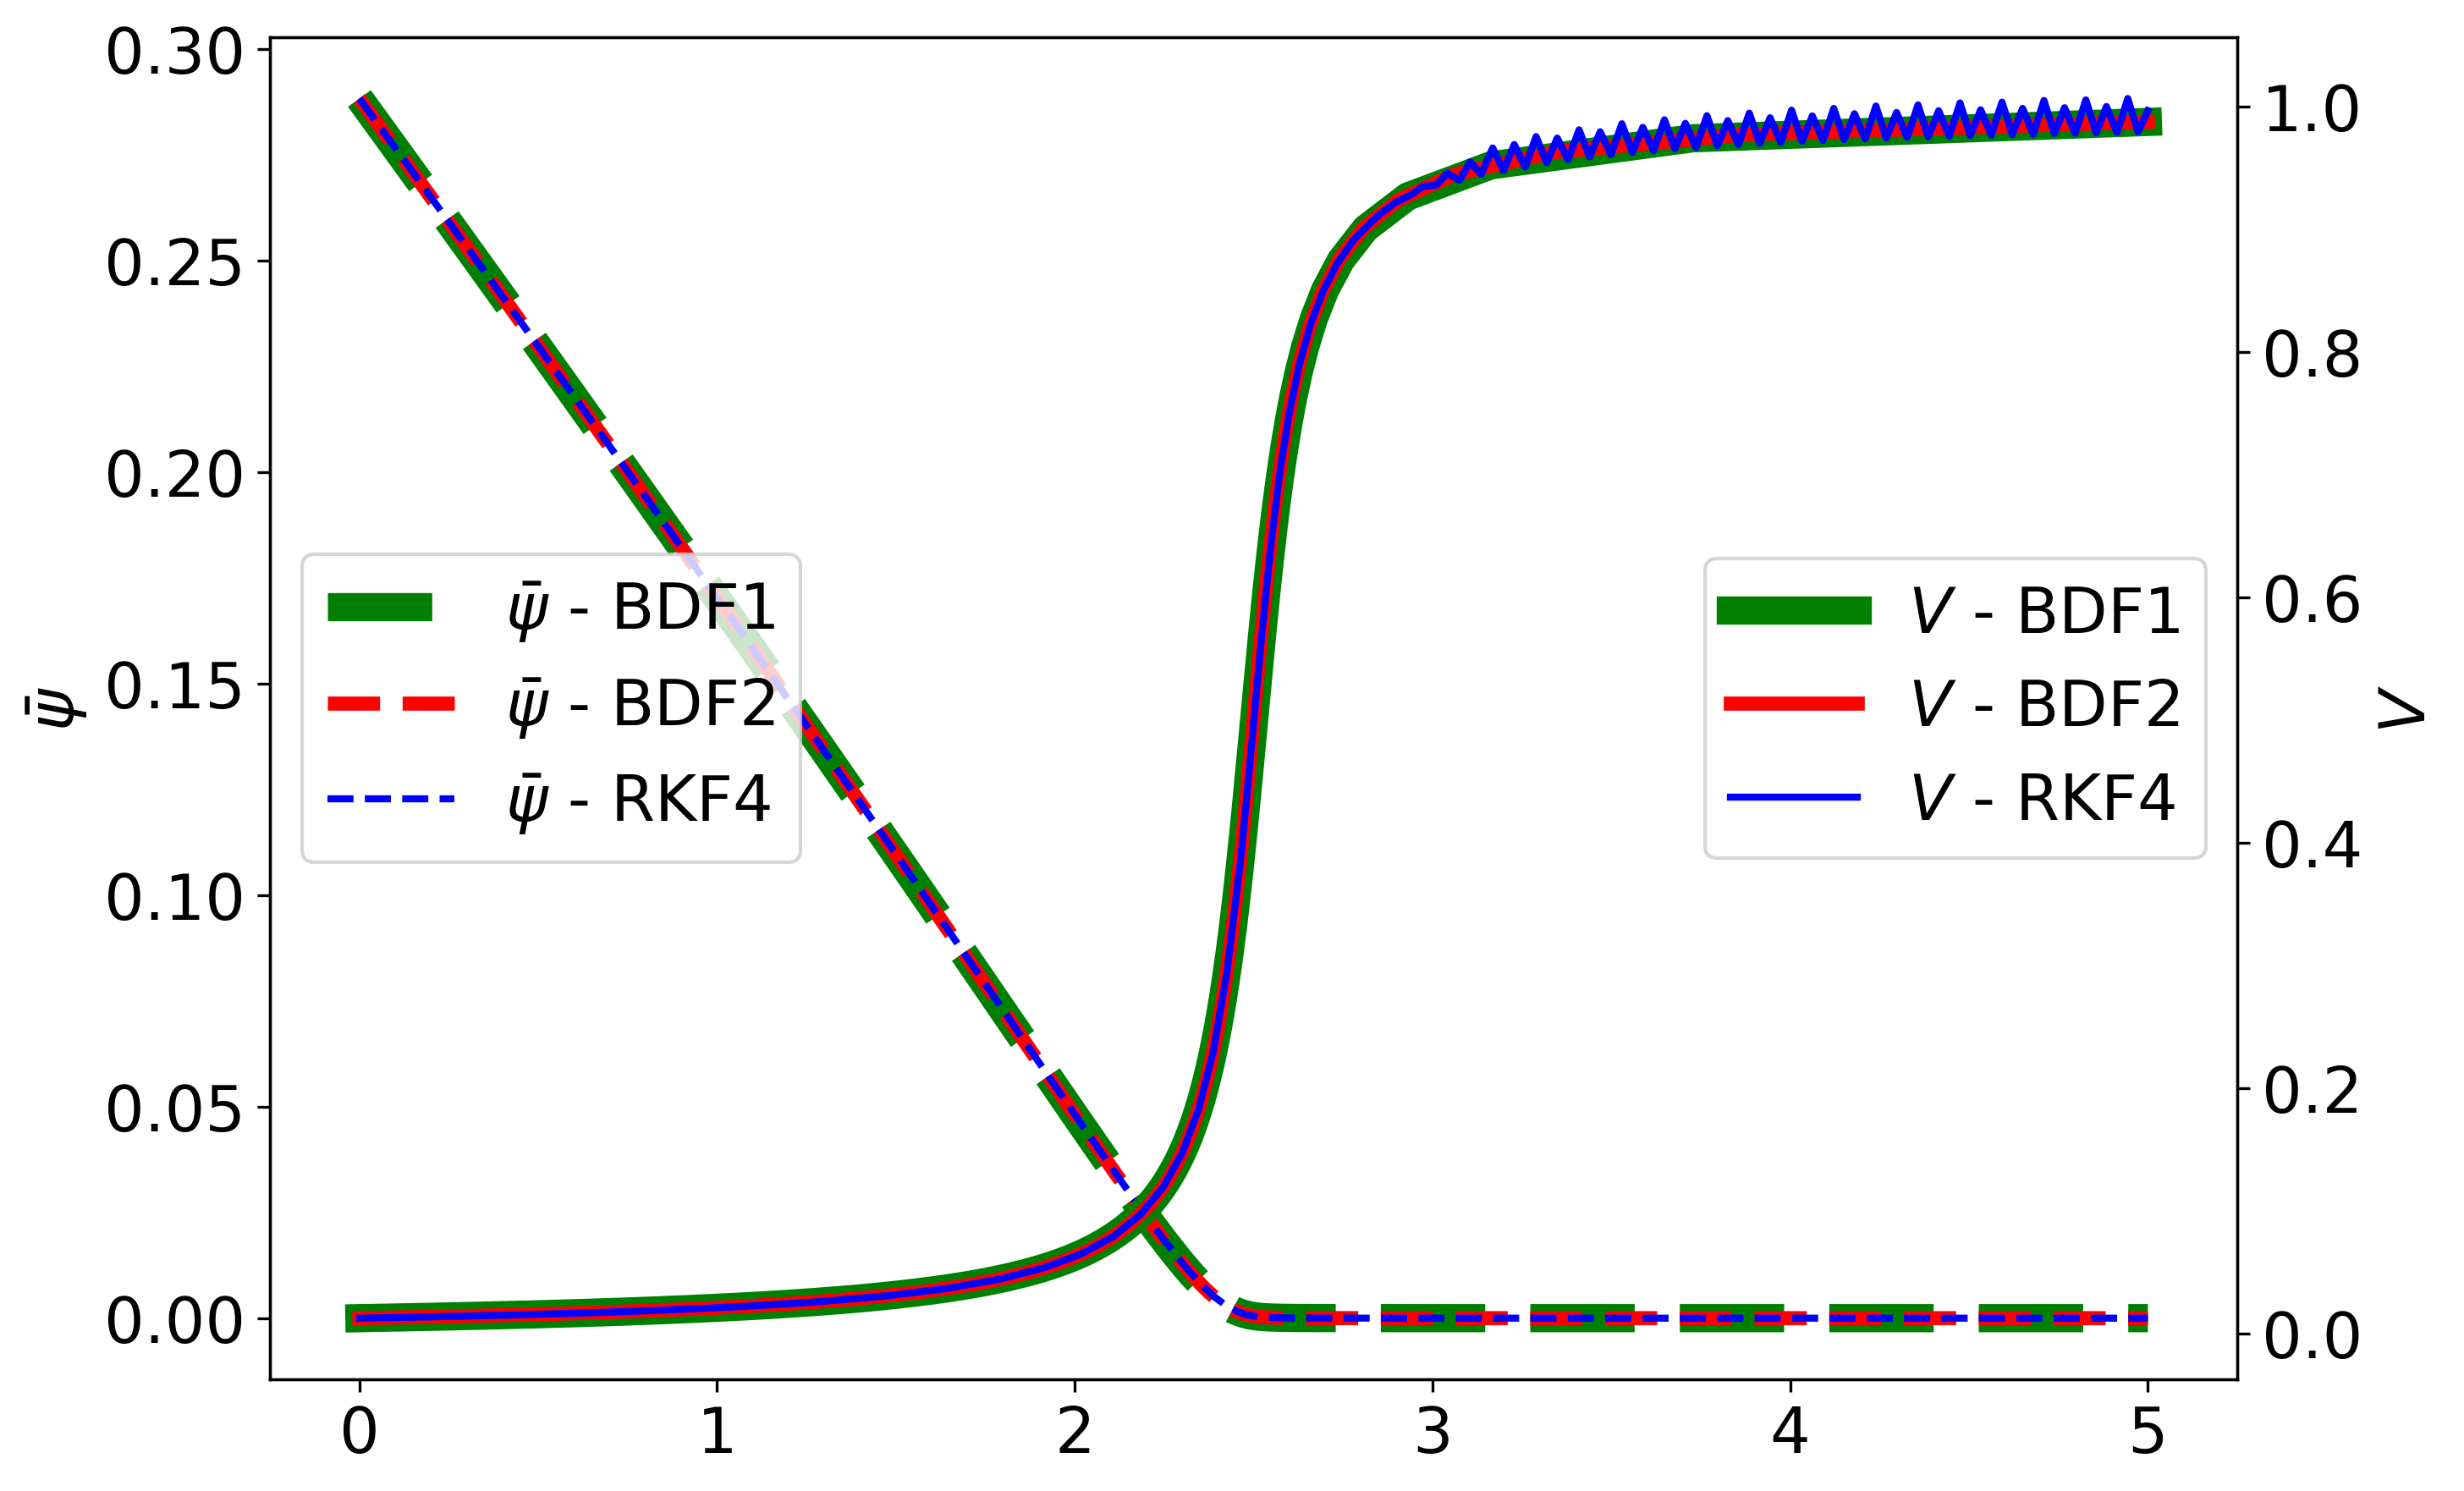
\includegraphics[width=1\textwidth]{images/timeEvolutionValues.png}
       	\subcaption{Evolution of the velocity $V$ and of the state variable $\bar{\psi}$} 
        \label{fig:timeEvolutionValues}
    \end{subfigure}
    \begin{subfigure}{0.43\textwidth}
    	\centering
    	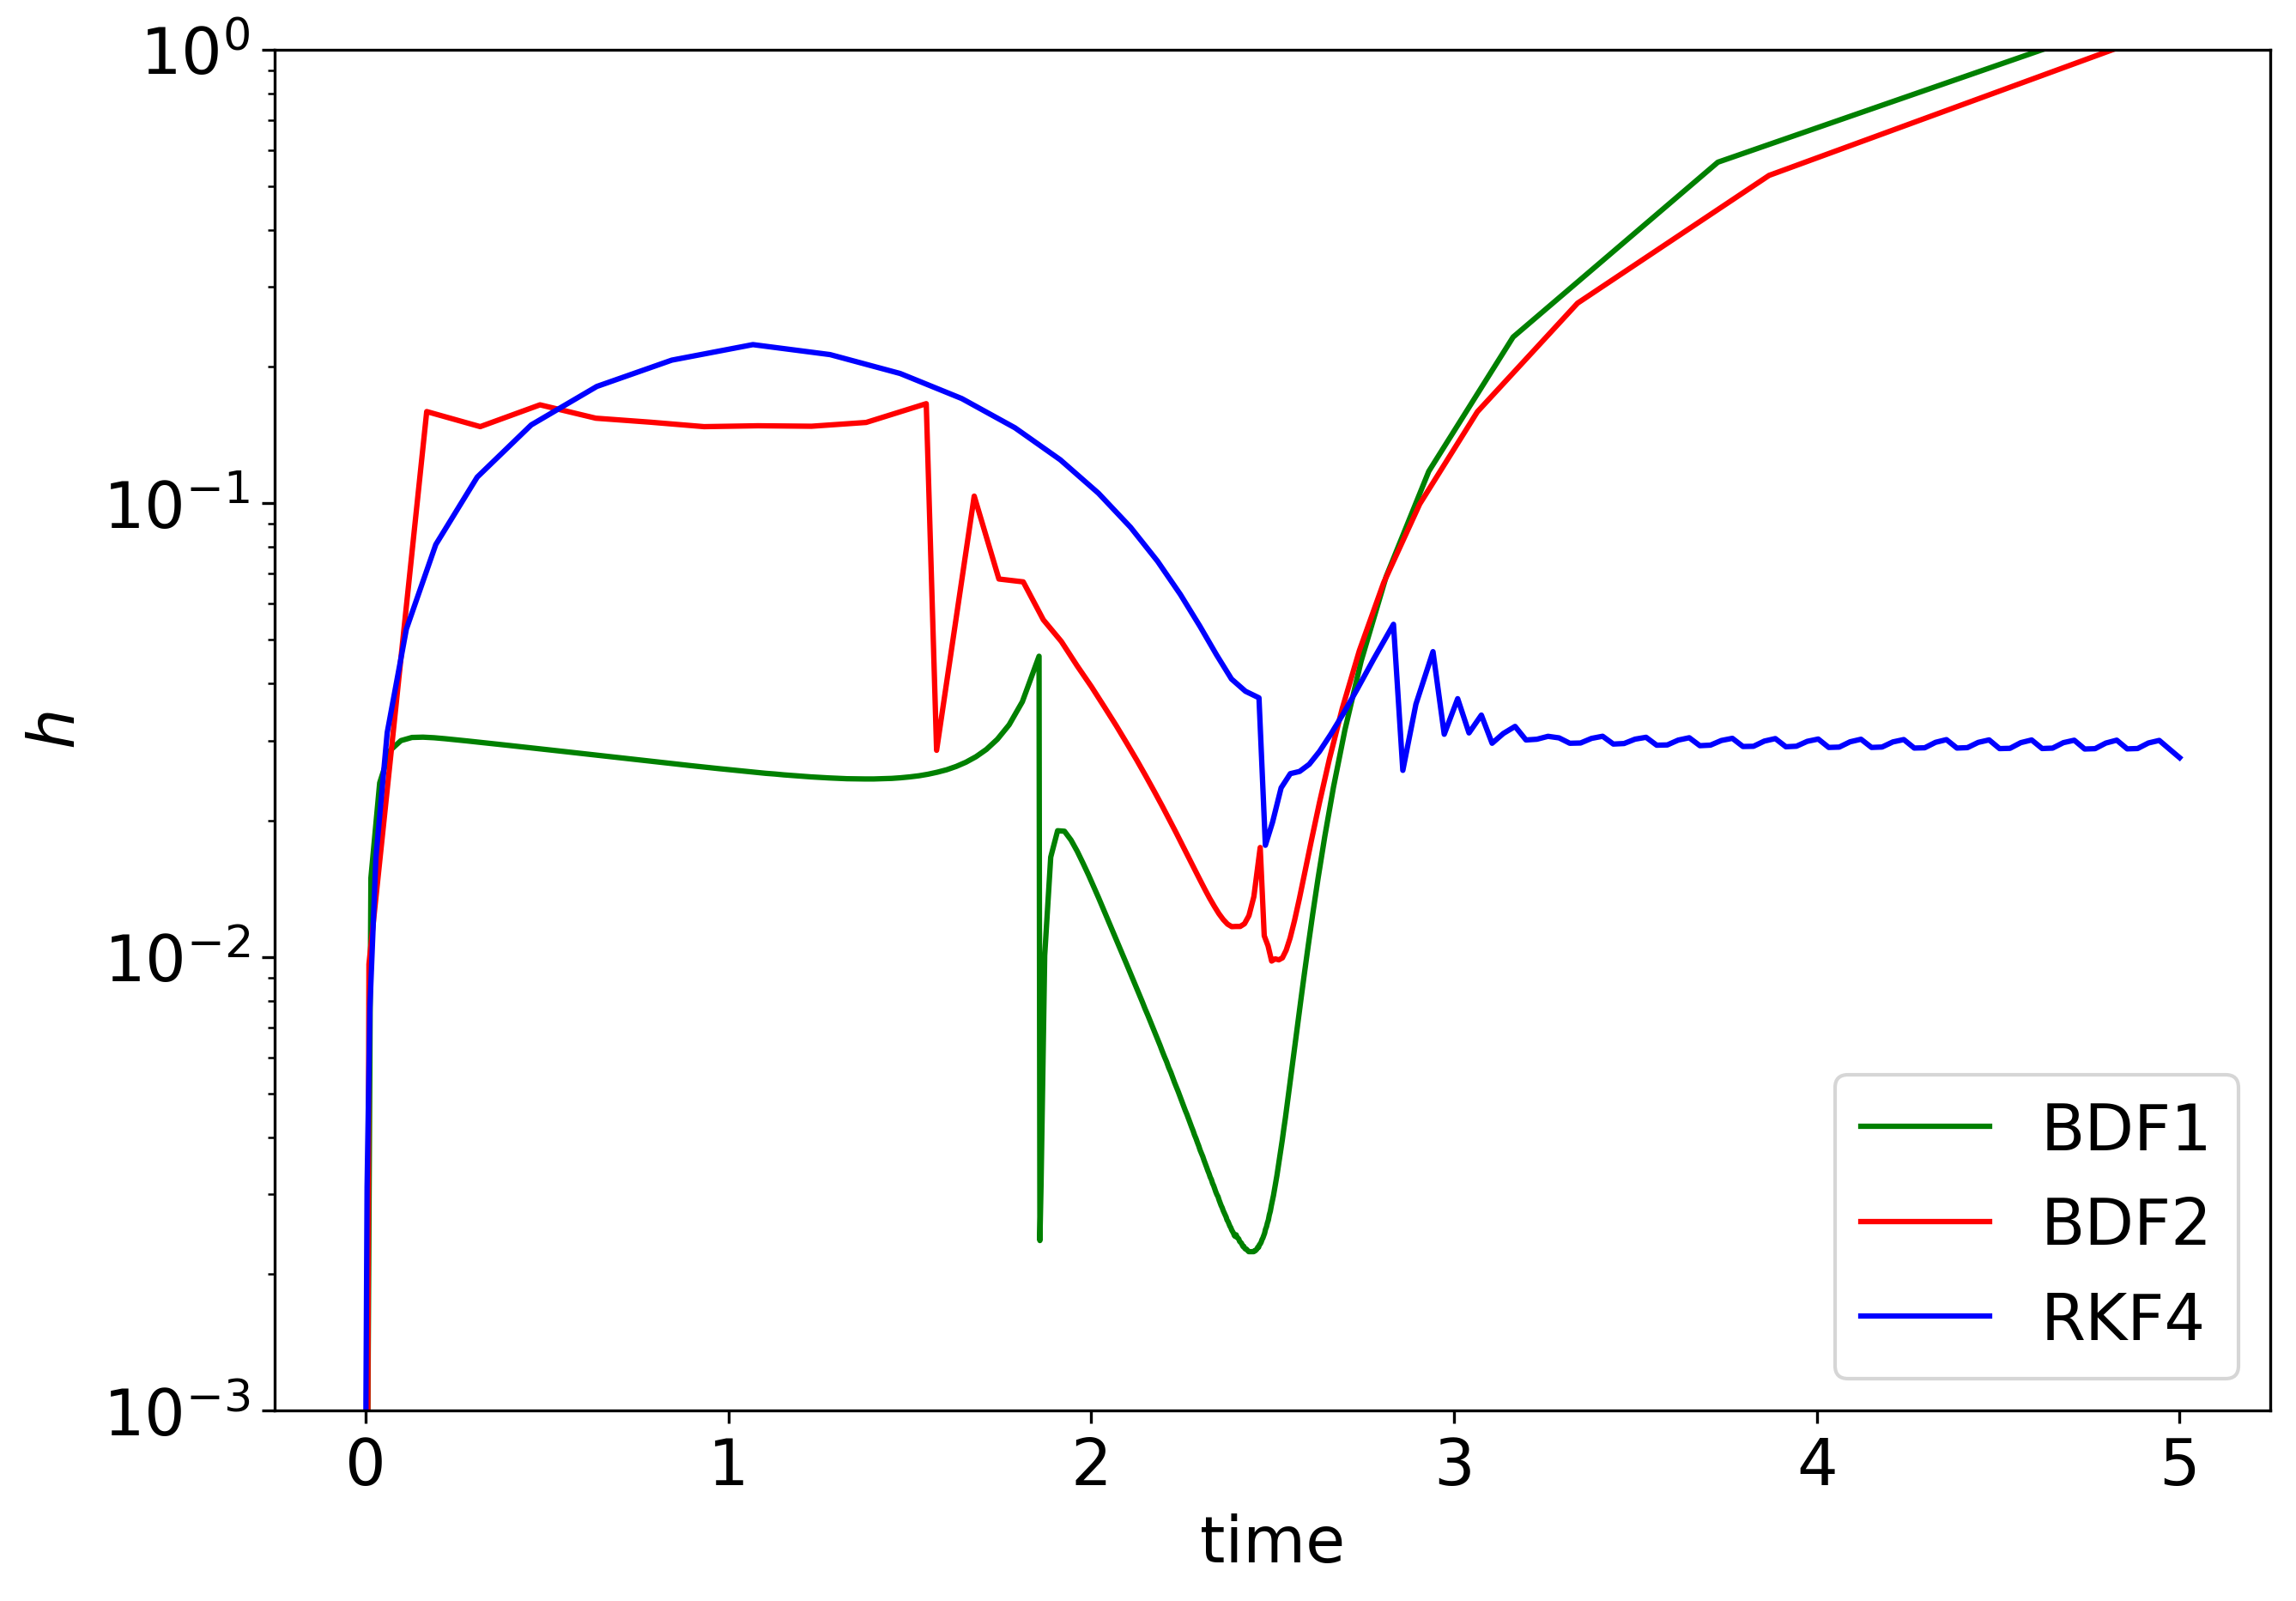
\includegraphics[width=1\textwidth]{images/timeEvolutionDT.png}
       	\subcaption{Evolution of the timestep size $h_n$} 
        \label{fig:timeEvolutionDT}
    \end{subfigure}
    \caption{Evolution of the solution and the timestep sizes of the single state problem defined in \autoref{eq:first_DAE_algeb} with the implemented numerical schemes}
\end{figure}
 
Now, the accuracy of the three numerical methods is compared. Therefore, the evolution of the absolute difference between the numerical solution and the analytical solution of the state variable $\bar{\psi}$ shown in \autoref{fig:timeEvolutionErrorPSI}. It is of interest to compare this error with the absolute error in velocity in \autoref{fig:timeEvolutionVerror}. \\ 
As $\bar{\psi}$ decreases, the error in $\bar{\psi}$ increases steadily for all three numerical solvers. The implicit BDF methods produce two peaks in the evolution of the error, the first shortly before the end of the decrease and the second at the transition of the velocity from 0 to 1. The norm of the error is much higher for \textbf{BDF1} than for \textbf{BDF2}, despite the lower number of timesteps of the latter. The explicit \textbf{RKF4} method produces a similar error norm as \textbf{BDF1}, but only in one peak at the beginning of the transition phase. At the end of the simulation, when $\bar{\psi}$ stays around 0, all solvers match closely with the analytical solution and the error remains very low. On the other hand, the error in the slip rate is very low for all solvers at the beginning and a peak in the error appears at the transition from 0 to 1. As usual, the highest error here appears for \textbf{BDF1}. Between the two remaining methods, \textbf{RKF4} has the lowest error and also allows larger timesteps. Nonetheless, it is of fourth order, whereas the explicit methods are only of first or second order. Towards the end of the simulation, the error in velocity obtained by the two implicit methods vanishes again, however \textbf{RKF4} produces suddenly very high errors which alternate between three different values. In \autoref{fig:timeEvolutionValues}, it can be seen that the velocity oscillates around the expected solution without getting closer to it. \\
\begin{figure}[H]
    \centering
    \begin{subfigure}{0.43\textwidth}
    	\centering
    	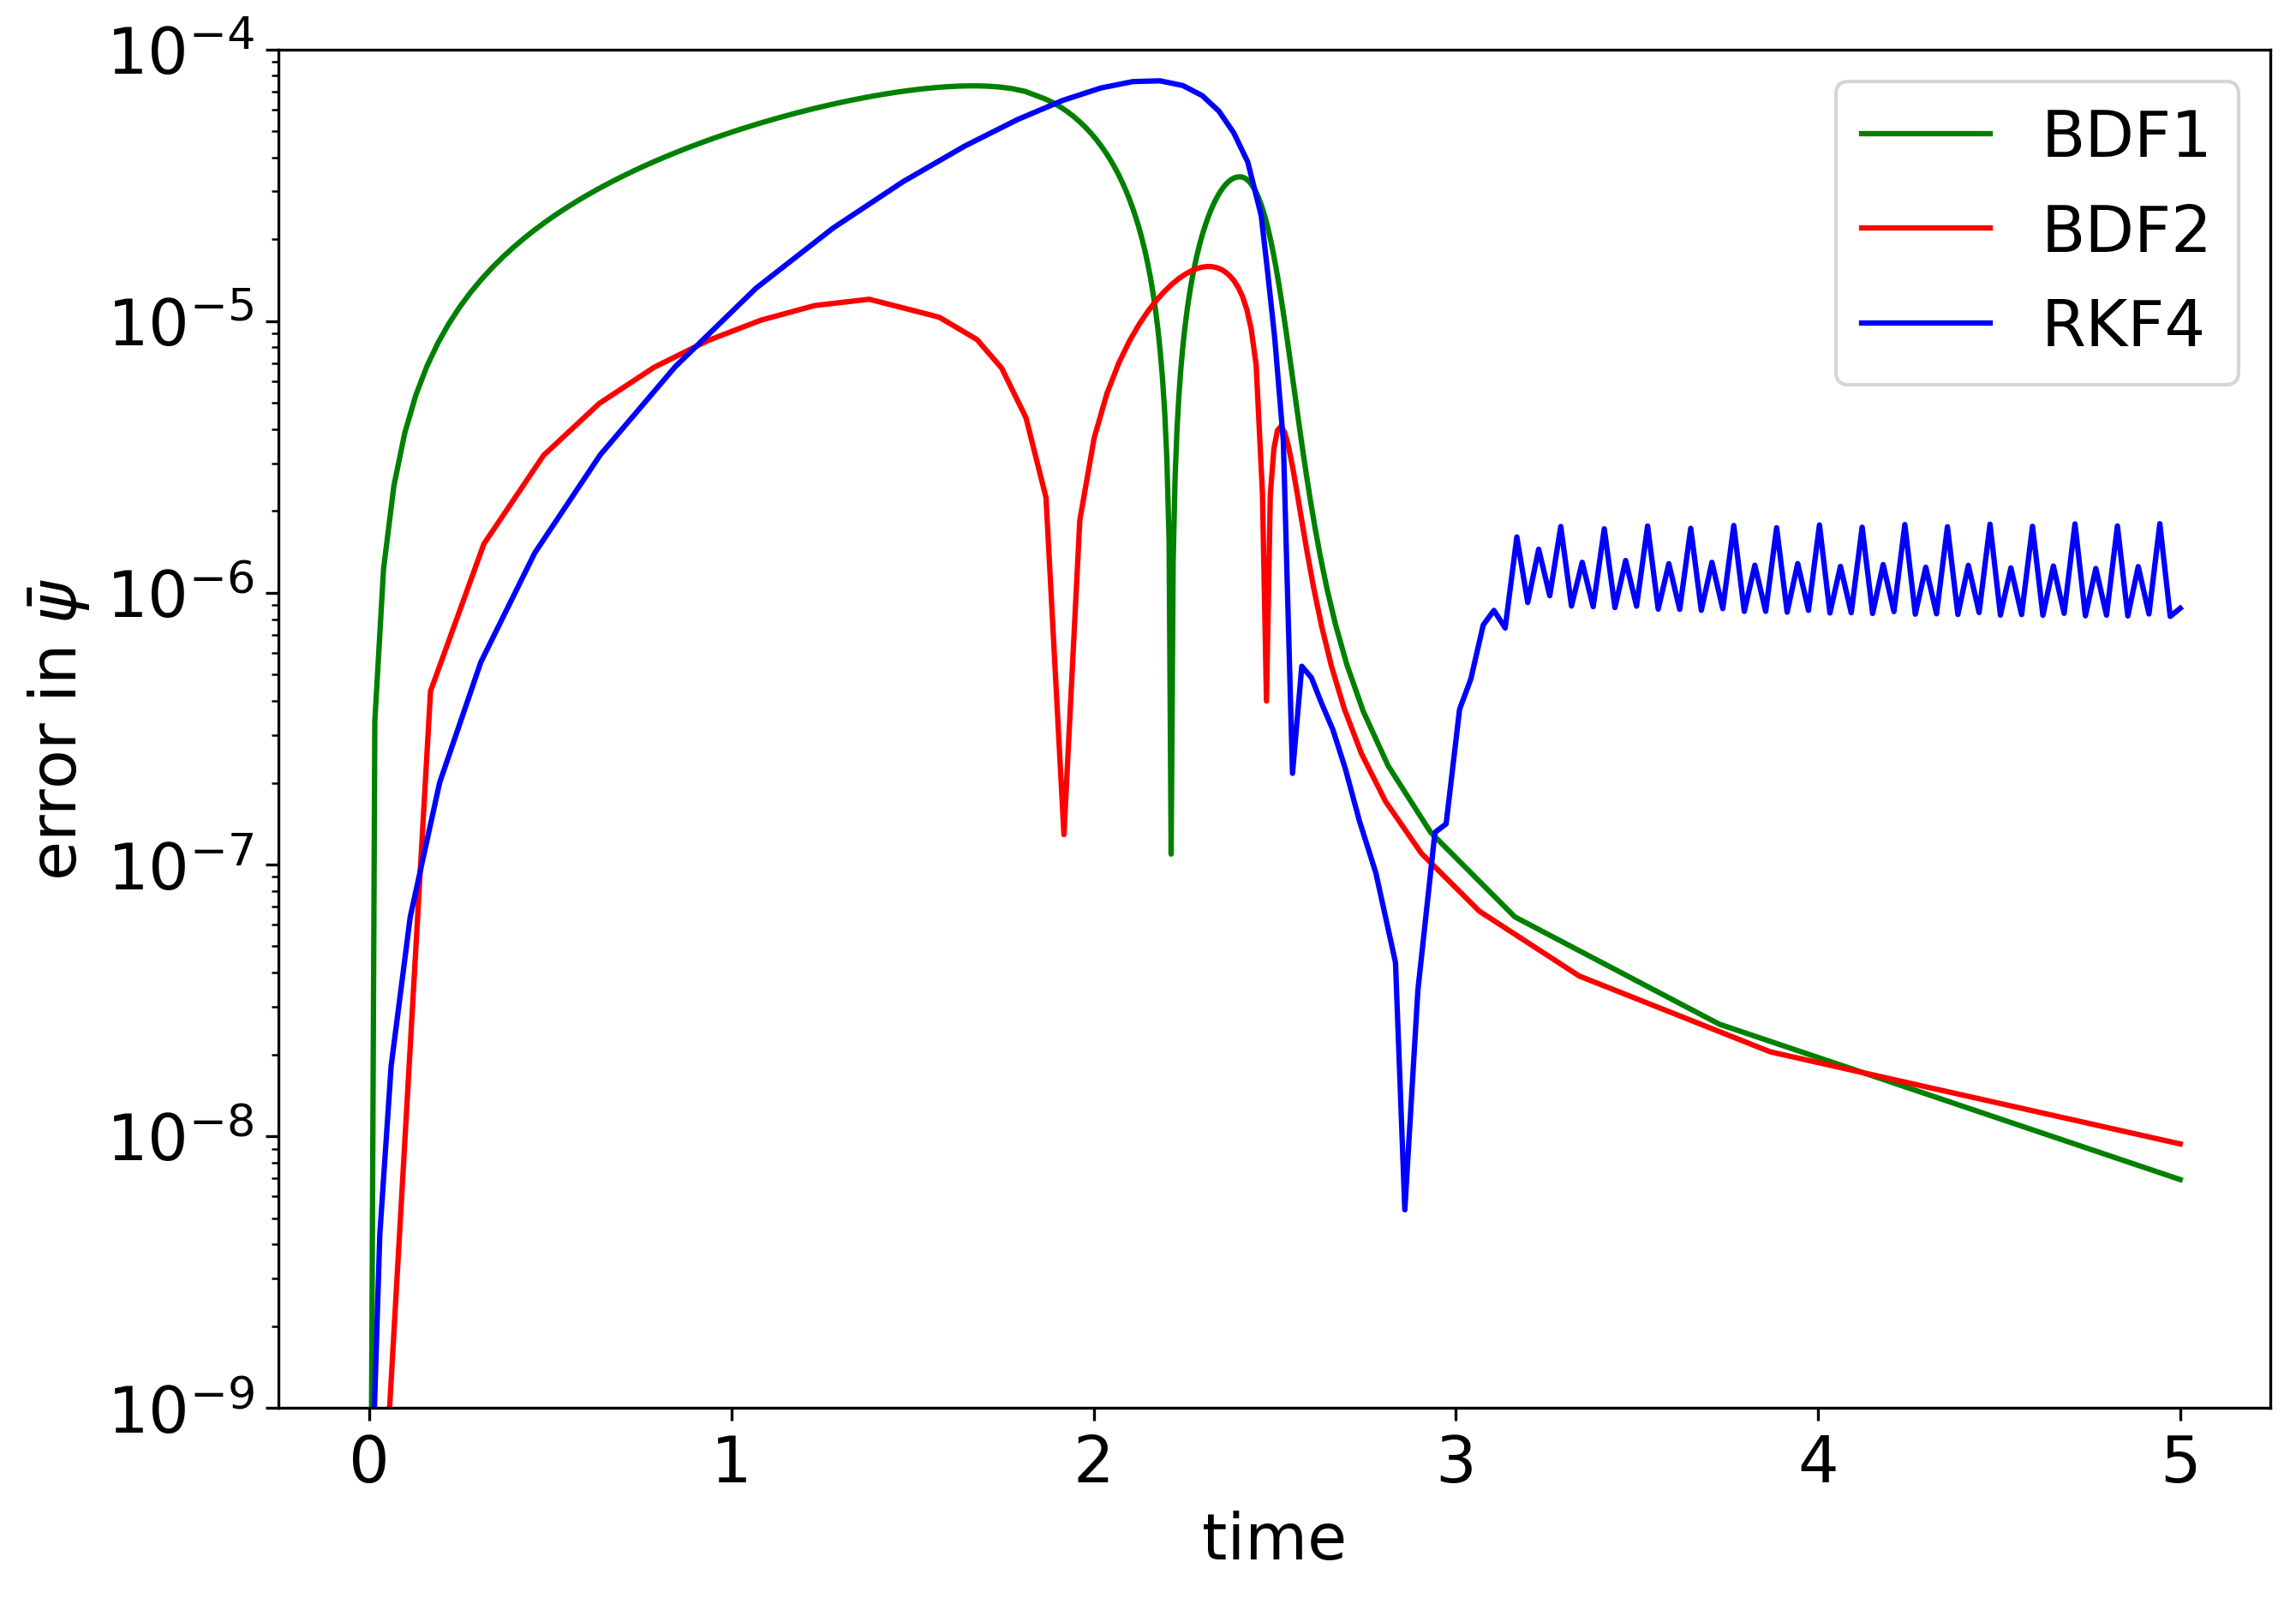
\includegraphics[width=1\textwidth]{images/timeEvolutionPSIerror.png}
       	\subcaption{Evolution of the absolute error of the state variable $\bar{\psi}$} 
        \label{fig:timeEvolutionErrorPSI}
    \end{subfigure}
    \begin{subfigure}{0.43\textwidth}
    	\centering
    	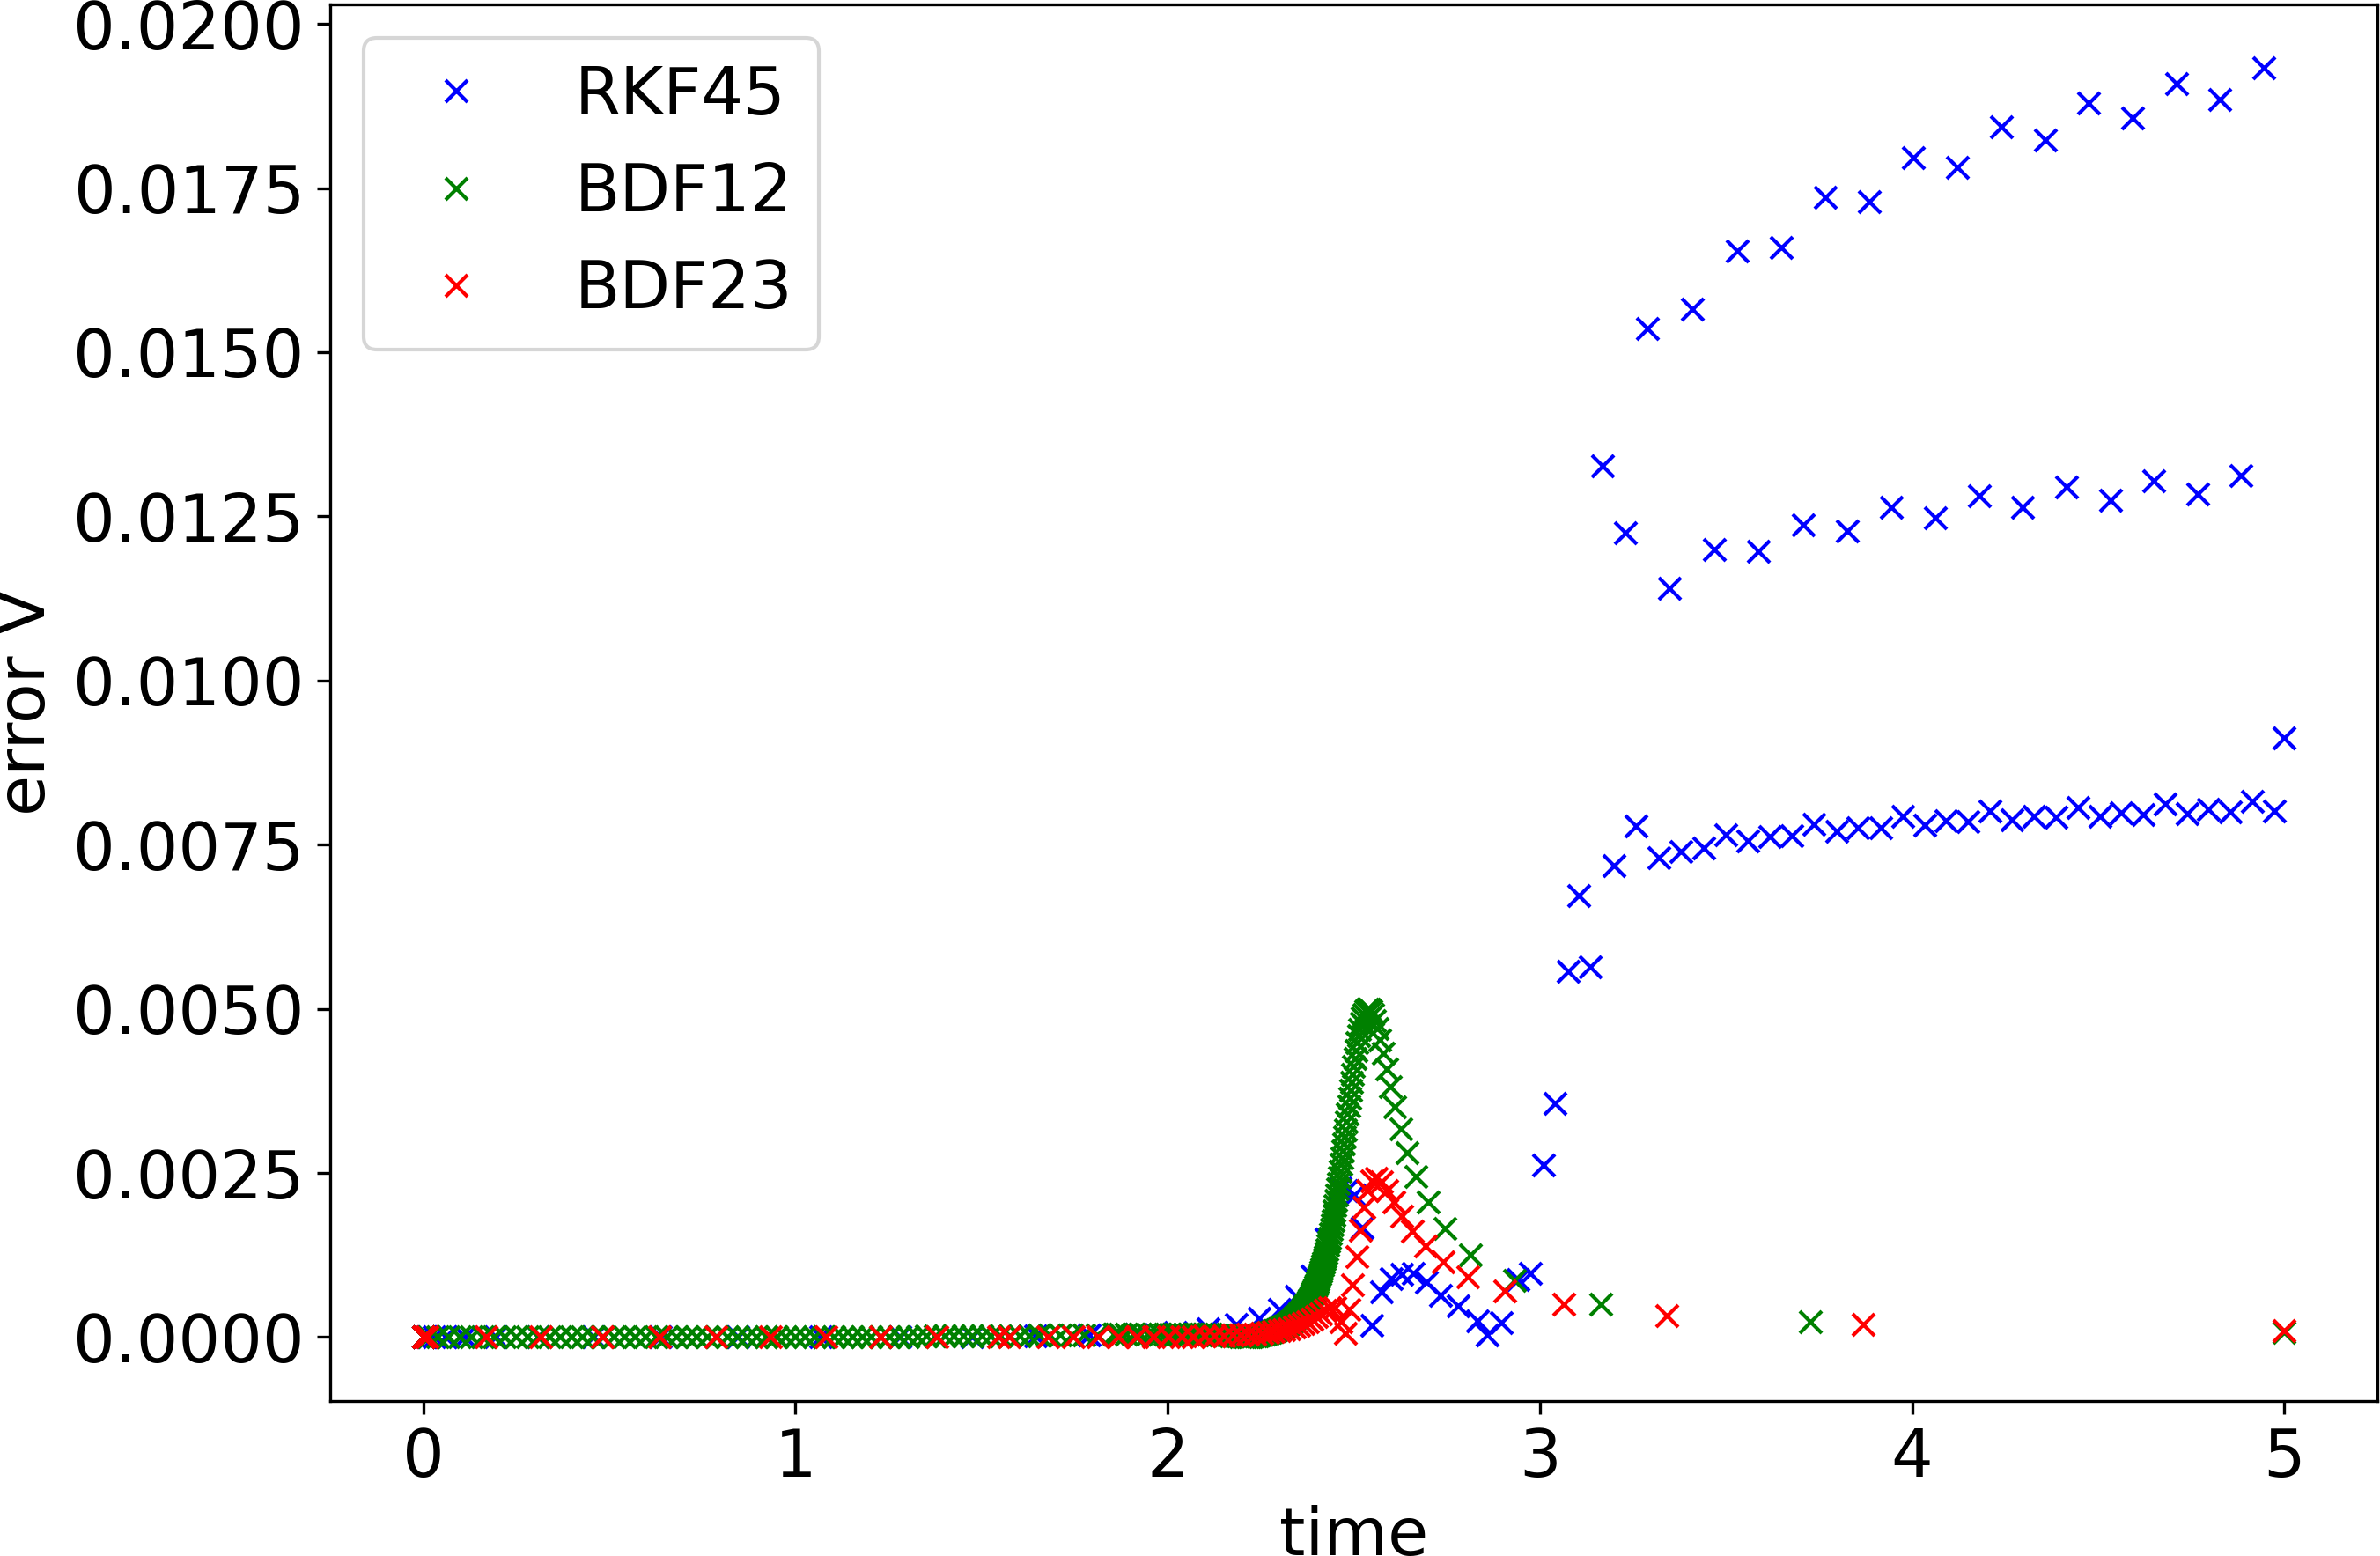
\includegraphics[width=0.95\textwidth]{images/timeEvolutionVerror.png}
       	\subcaption{Evolution of the absolute error of the velocity $V$ \\ \ } 
        \label{fig:timeEvolutionVerror}
    \end{subfigure}
    \caption{Evolution of the error for the single state problem defined in \autoref{eq:first_DAE_algeb} with the implemented numerical schemes}
\end{figure}

It is important to consider that the error in $\bar{\psi}$ and the velocity are not directly correlated, thus a small error in $\bar{\psi}$ does not necessarily lead to a small error in the velocity. It might therefore be wise to reconsider the way the timestep size is controlled. So far, it only depends on the ratio between the local truncation error and a predefined tolerance value. This error is estimated by applying another numerical scheme with higher order, by taking the difference in $\bar{\psi}$ of the two solutions as an error estimate. Therefore, the velocity is not involved in the step size controller and the controller cannot ensure that the chosen timestep size guarantees sufficiently accurate results for the velocity. To ensure correct physical results, the controller needs to be extended in a way to restrict the timestep size depending on some error estimate of the velocity. 

\subsection{Quality of the error estimates}
\label{ssec:QualityErrorEstimate_0D}
The whole theory of timestep controllers is based on an accurate error estimate, which is obtained in our case by calculating the solution with a higher order method. It is interesting to analyze whether the error estimate calculated in this way matches the actual error to the analytical solution. The absolute error cannot be used like in the previous graphs, since the error estimate is calculated from the lower-order solution at the previous timestep. On the other hand, the local truncation error, which measures by how much the total error increases at each timestep, is much better suited to evaluate the accuracy of the error estimate. \\
In \autoref{fig:errorEstimateEvolutionALL}, the difference between the two solutions calculated at each timestep with any of the schemes, being the error estimate, is plotted against the real local truncation error. In the initial phase, the two implicit methods estimate the error very closely to its real value. Even though the \textbf{BDF1} method approximates it better than the \textbf{BDF2} method, the high number of needed timesteps in this phase increases the total error which turns out to be much worse. The estimate of the explicit \textbf{RKF4} method roughly follows the real evolution of the local truncation error but underestimates it by a large factor up to 5. During the transition phase, the situation is reversed, because the implicit methods fail at estimating correctly peaks in the evolution of the real error and remain instead around the same value. On the other hand, the \textbf{RKF4} better fits the evolution of the local truncation error, which explains its good performance in the transition phase. In the final phase, the two implicit methods match again with the expected error values and the \textbf{RKF4} method seems to fit exactly the real error, but it shows nonphysical oscillations which seem to correspond to the larges oscillations in the total error of the velocity. \\
Overall, implicit methods yield better error estimates except for the transition which seems to be better handled by the explicit scheme. 

\begin{figure}[H]
    \centering
    \begin{subfigure}{0.32\textwidth}
    	\centering
    	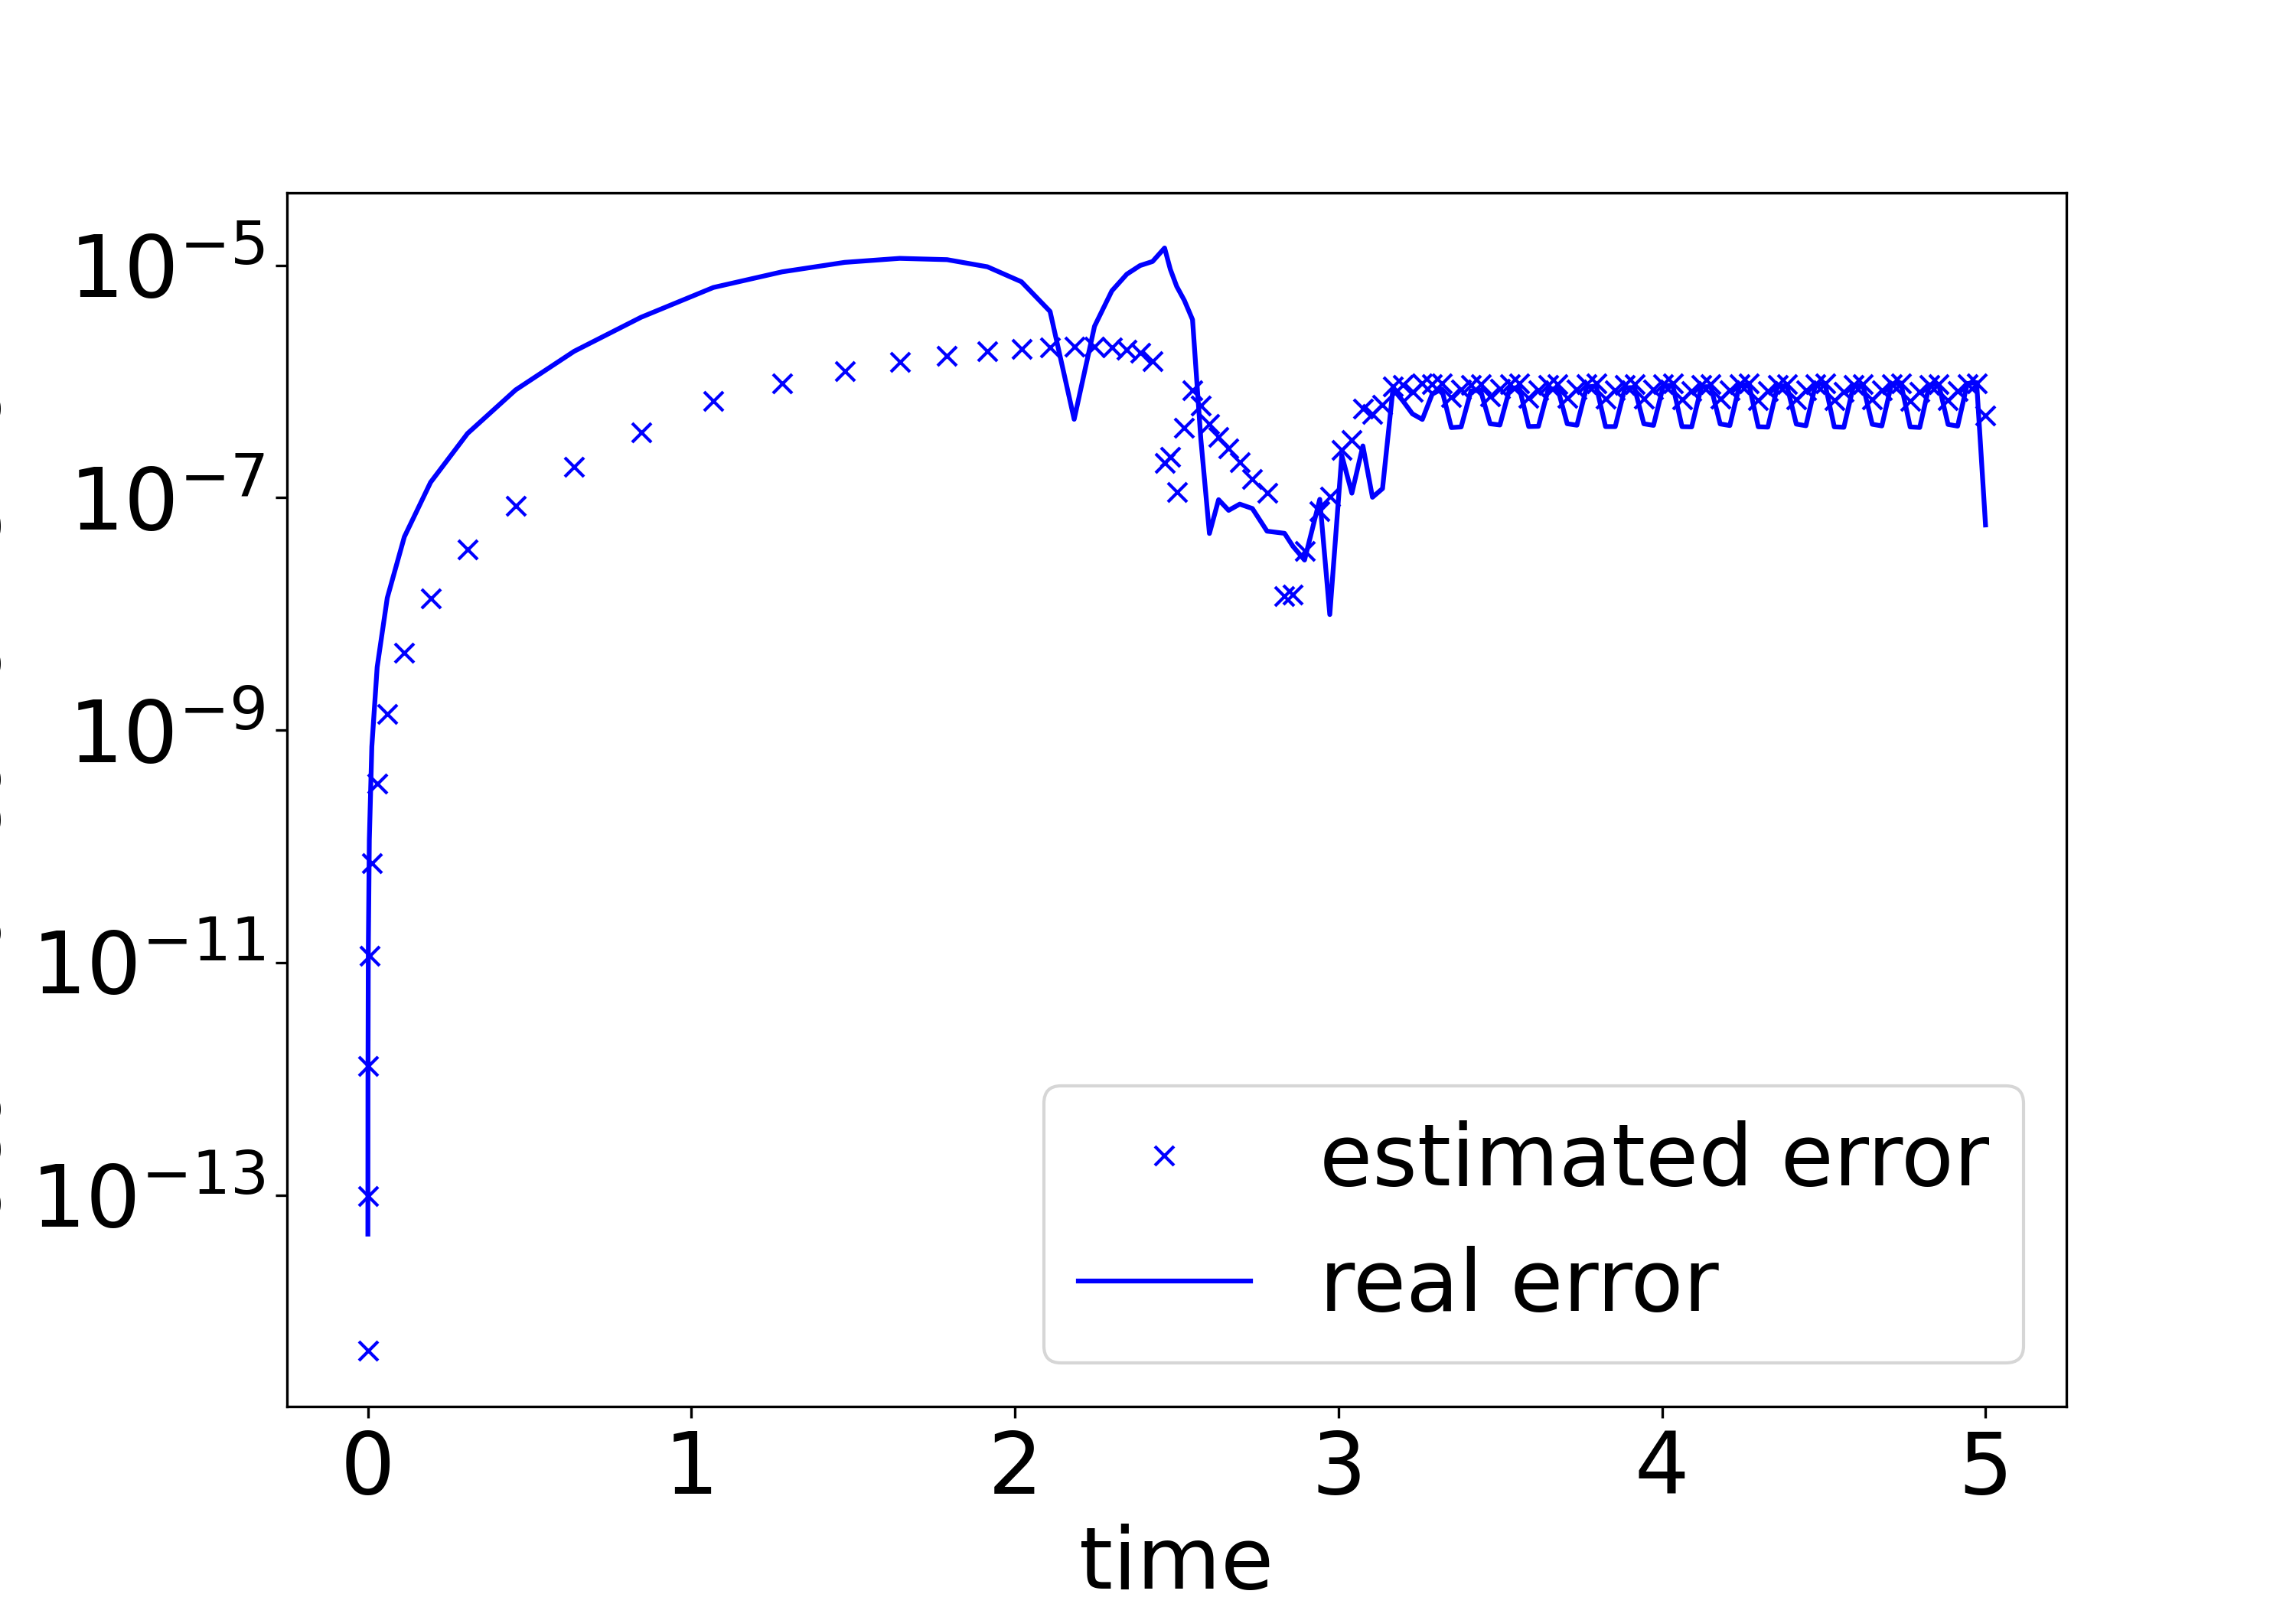
\includegraphics[width=1\textwidth]{images/errorEstimateRKF45.png}
       	\subcaption{\textbf{RKF4}} 
        \label{fig:errorEstimateEvolutionRKF45}
    \end{subfigure}
    \begin{subfigure}{0.32\textwidth}
    	\centering
    	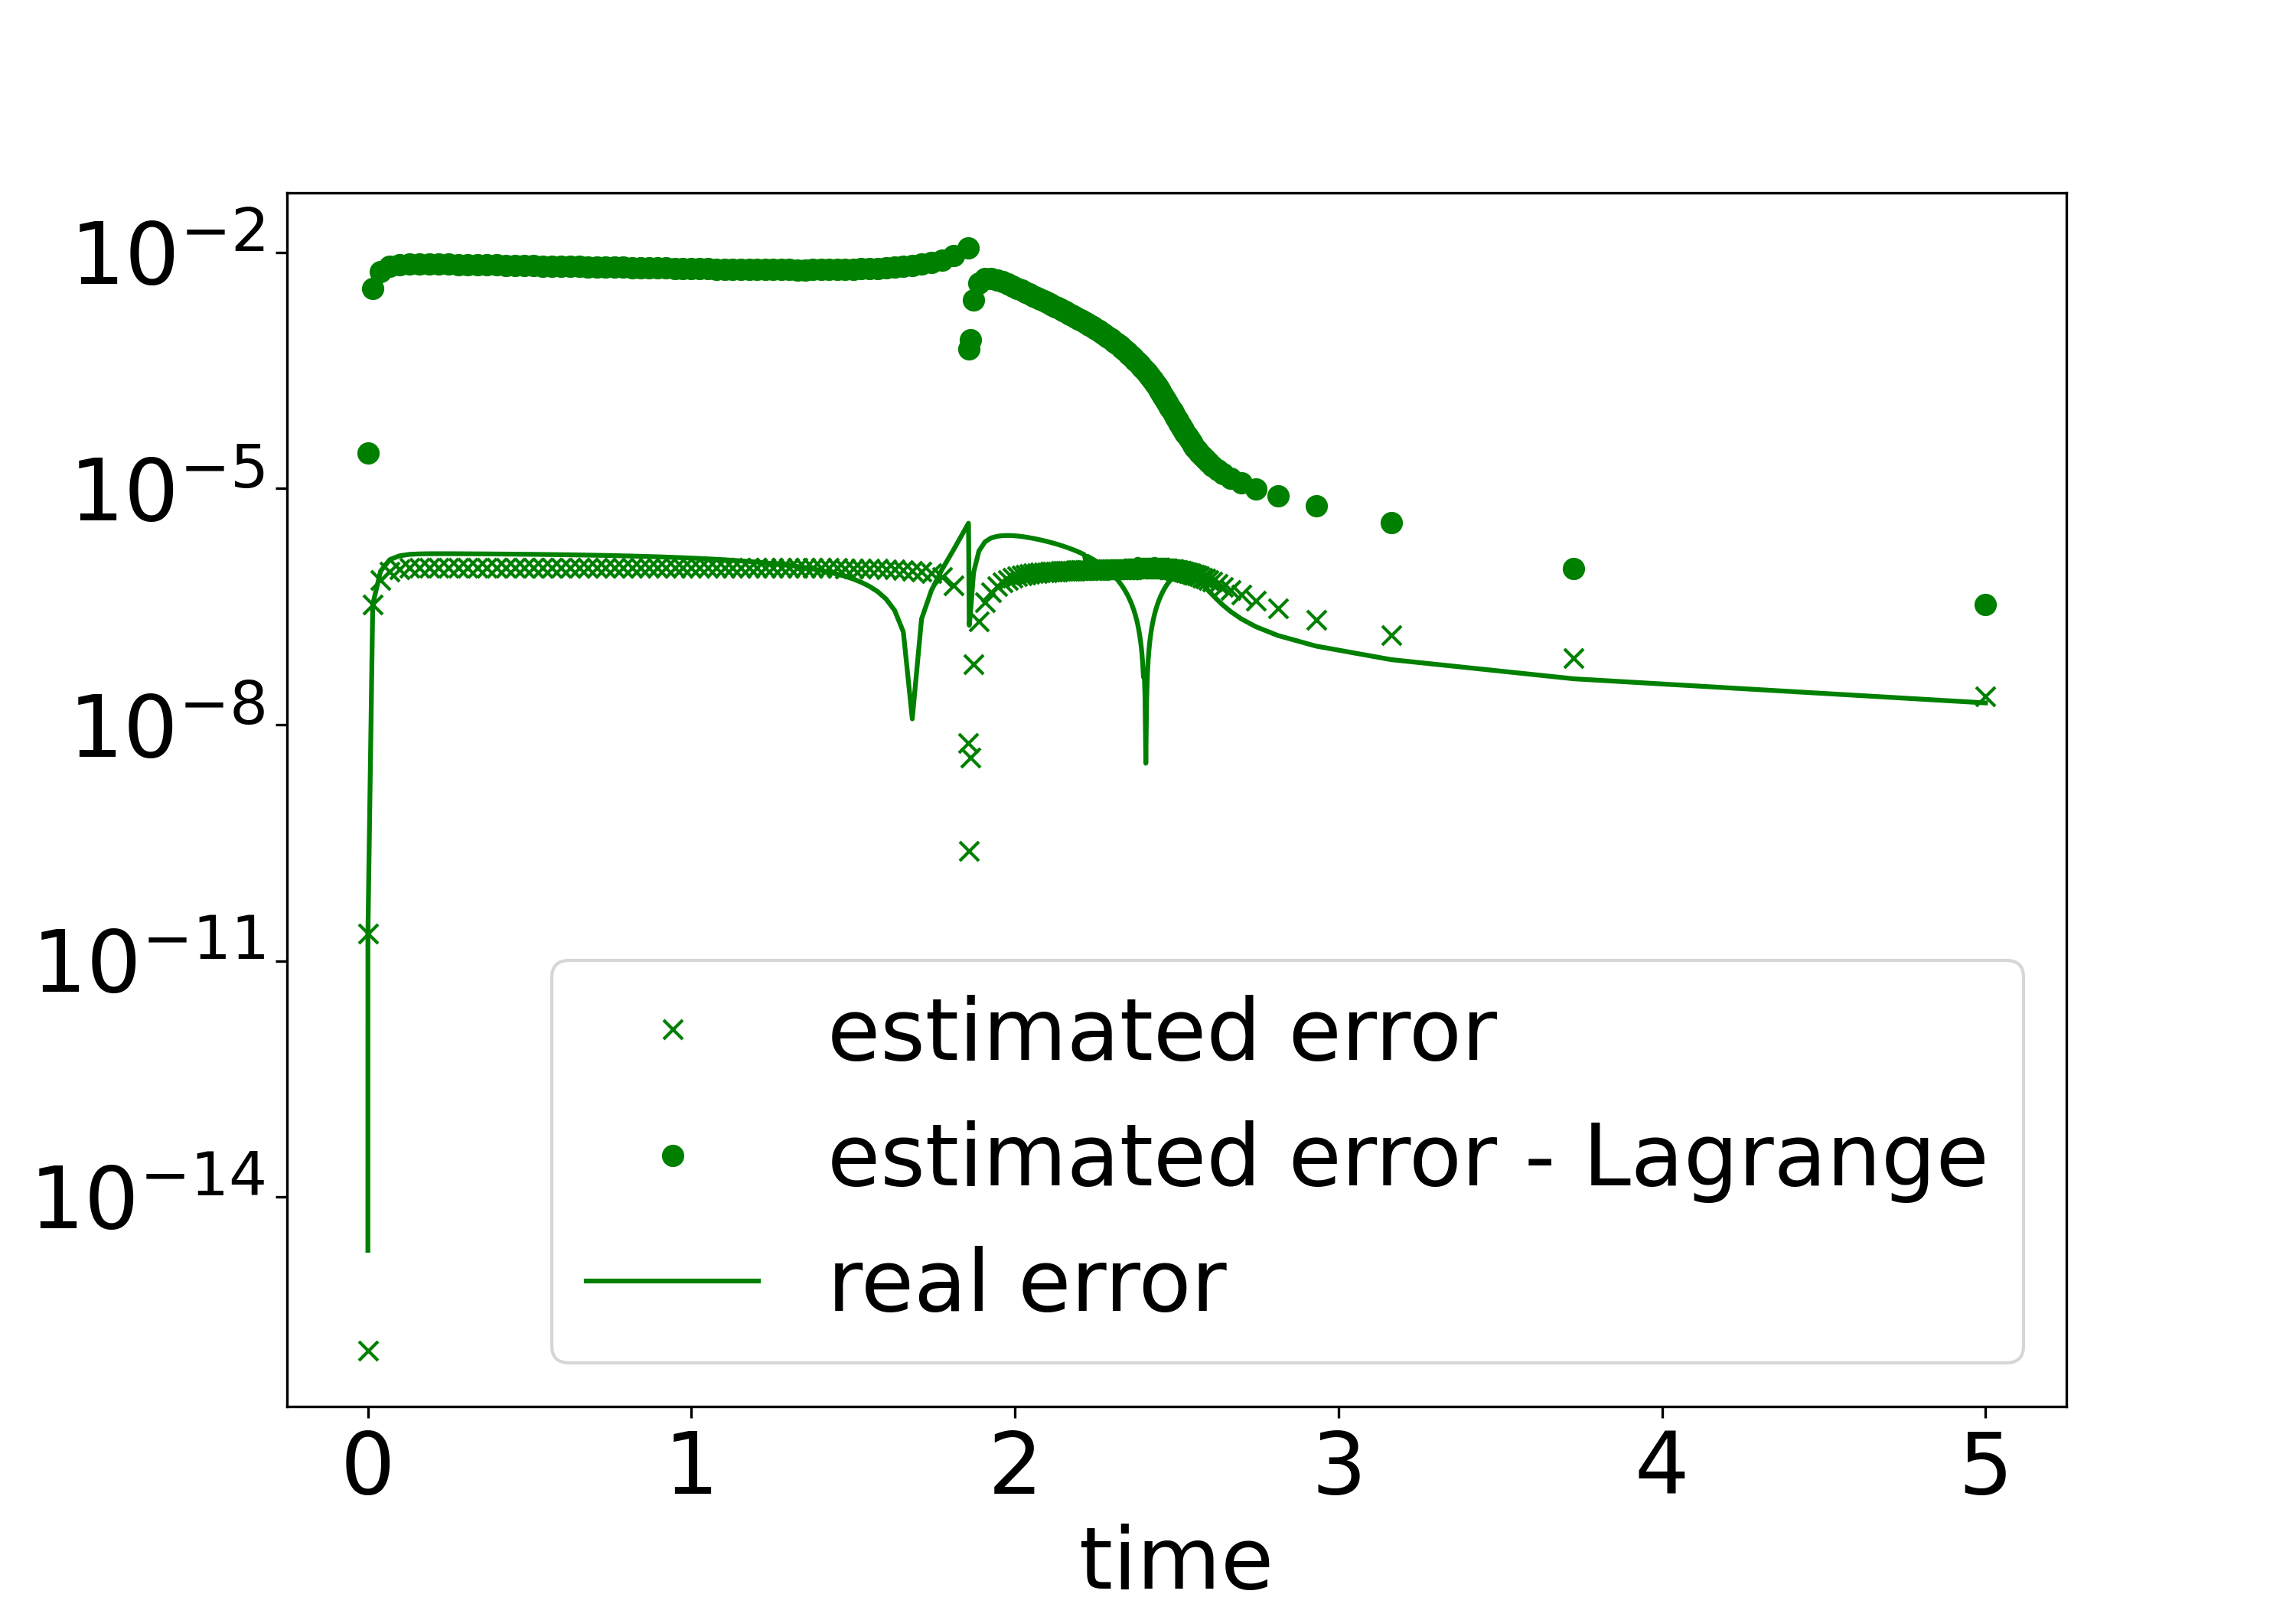
\includegraphics[width=1\textwidth]{images/errorEstimateBDF12.png}
       	\subcaption{\textbf{BDF1}} 
        \label{fig:errorEstimateEvolutionBDF12}
    \end{subfigure}
    \begin{subfigure}{0.32\textwidth}
    	\centering
    	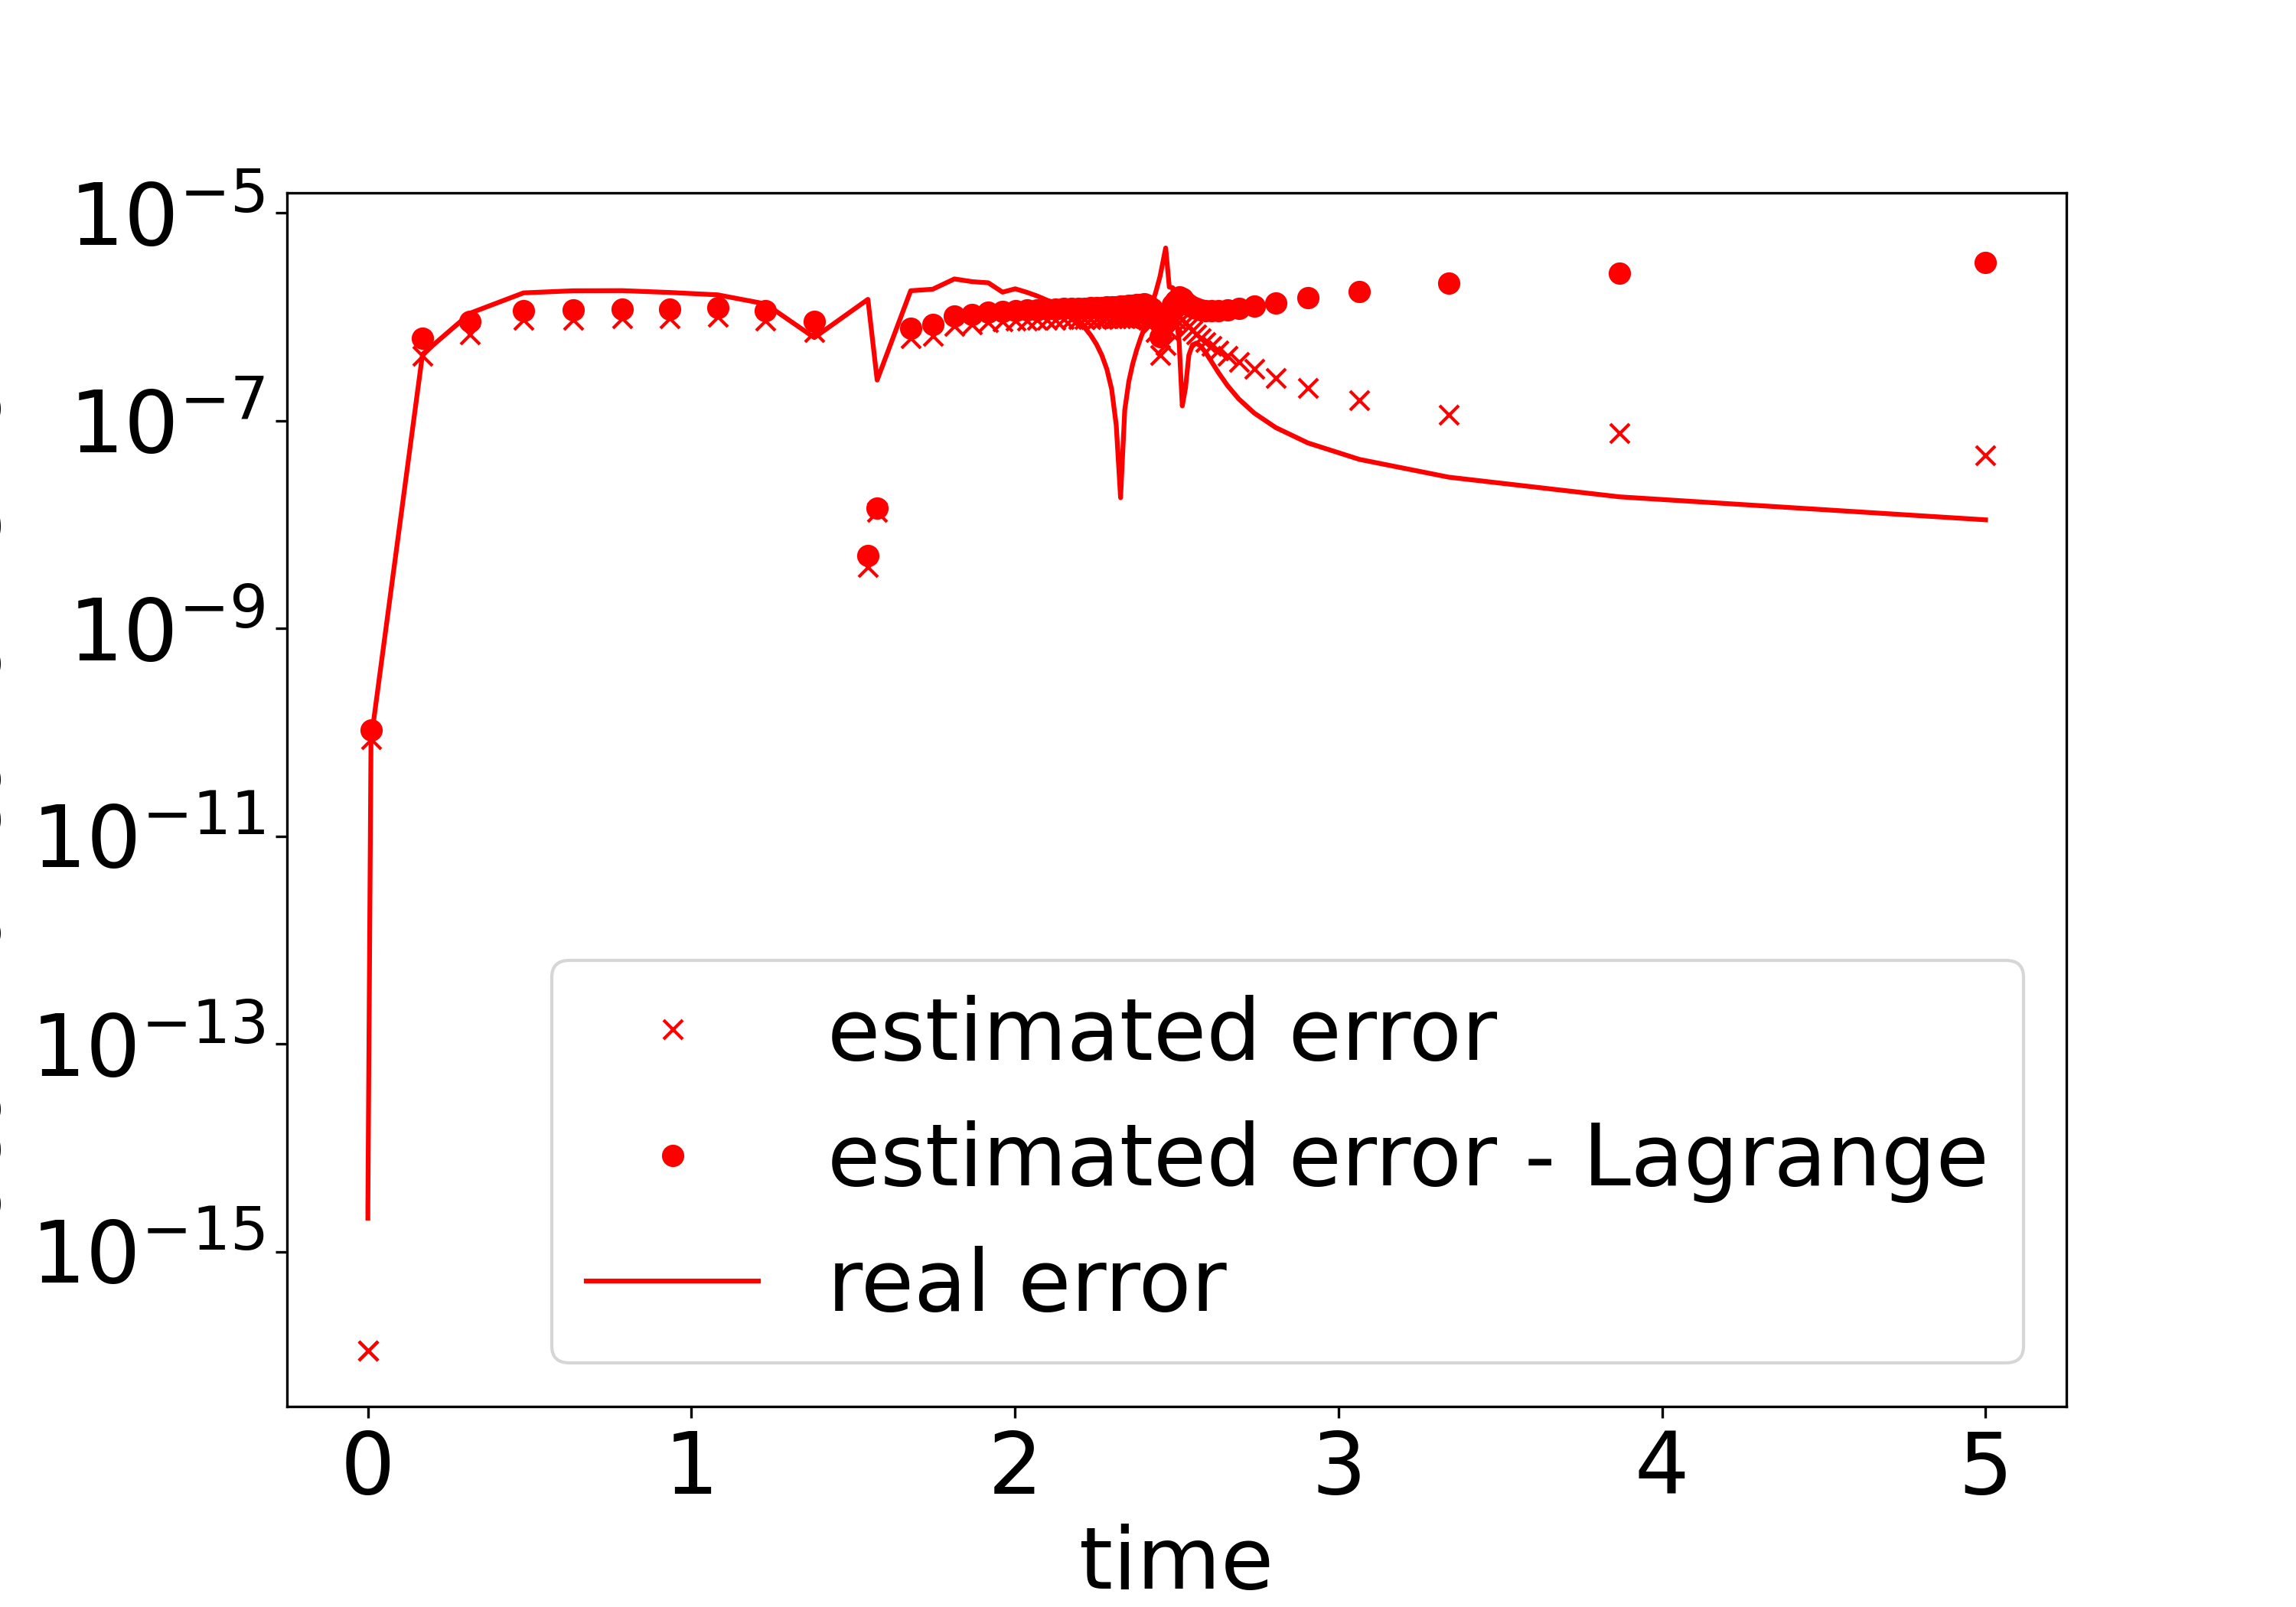
\includegraphics[width=1\textwidth]{images/errorEstimateBDF23.png}
       	\subcaption{\textbf{BDF2}} 
        \label{fig:errorEstimateEvolutionBDF23}
    \end{subfigure}
    \caption{Evolution of the local truncation error and of the error estimate for the single state problem defined in \autoref{eq:first_DAE_algeb} with the implemented numerical schemes}
    \label{fig:errorEstimateEvolutionALL}
\end{figure}
\newpage
For BDF methods, two error estimates have been introduced: with a higher order evaluation of the solution and using the derivative of the Lagrange interpolation. For \textbf{BDF1}, the embedded estimate is much closer to the real error as the Lagrange method indicates an error several orders of magnitude too large. For \textbf{BDF22}, this difference diminishes but is still significant. The problem of a too large estimated error is, that the timestep controller restricts wrongly the timestep size. On the other hand, the embedded error estimate is much more expensive to evaluate, so it is only worth if it allows timestep sizes that are at least twice as large as with the Lagrange error estimate. The effect on the total number of timesteps of both approaches will be investigated in detail in \autoref{sec:Results_BDFOrder}. \\

In conclusion, the implicit \textbf{BDF2} method gives the best results because overall, the induced total error remains low, it allows for the highest timestep sizes and the local truncation error is generally well estimated. In contrast, the \textbf{BDF1} method is restricted to much smaller timesteps which makes it unattractive for most simulations. Another negative side effect of the small timesteps is the large difference to the analytical solution since the local errors accumulate steadily. The explicit \textbf{RKF4} fails if the velocity is too high, so it should not be used in such cases. However, it has a strong advantage over the \textbf{BDF2} method for very small velocities because it allows for larger timesteps. Additionally, it better estimates the local truncation error in the transition phase from low to high velocities.
